\documentclass[output=paper,colorlinks,citecolor=brown,chinesefont]{langscibook}
\ChapterDOI{10.5281/zenodo.15148180}
\author{Thom van Hugte\orcid{}\affiliation{Leipzig University} and         Yiya Chen\orcid{}\affiliation{Leiden University} and        Li Guo\orcid{}\affiliation{Shanghai International Studies University}}

\title{The contradictory nature of fricative vowels in Chinese and beyond}

\abstract{This chapter is concerned with fricative vowels, an umbrella term for speech sounds that are syllabic but nevertheless typically involve frication so that they are difficult to categorise as either consonants or vowels. Because of these contradictory properties and their overall rarity, there are many different terms for fricative vowels and there is a general lack of awareness among linguists that these sounds exist. Very few studies have attempted to compare fricative vowels cross-linguistically, but it is clear that there are both similarities and differences among them. The goal of this chapter is to provide an overview of fricative vowels and of the major descriptive and theoretical questions that they raise.

\keywords{fricative vowels, vowel fricativisation, Sinitic languages, manner of articulation}
}

%move the following commands to the "local..." files of the master project when integrating this chapter
\usepackage{tabularx}
\usepackage{langsci-optional}
\usepackage{langsci-gb4e}


\IfFileExists{../localcommands.tex}{
   \addbibresource{../localbibliography.bib}
   \usepackage{tabularx, multicol, multirow, longtable}
\usepackage{url}
\urlstyle{same}

\usepackage{orcidlink}
\definecolor{orcidlogocol}{cmyk}{0,0,0,1}
\RenewDocumentCommand{\LinkToORCIDinAffiliations}{ +m }
  {%
    \orcidlink{#1}\,%
  }
\SetupAffiliations{orcid placement=before}

\usepackage{siunitx}
\sisetup{detect-weight=true, detect-family=true, group-digits=none}

\usepackage{mathtools}
\usepackage{langsci-optional}
\usepackage{langsci-lgr}
\usepackage{langsci-gb4e}

\usepackage{stmaryrd}
\usepackage[capitalize]{cleveref}
\babelfont[macedonian]{rm}[Language=Macedonian,ItalicFont=LibertinusSerif-Italic.otf]{LibertinusSerif-Regular.otf}
\usepackage{eqparbox}
\usepackage[autostyle]{csquotes}
\usepackage[linguistics]{forest}

\usetikzlibrary{positioning, matrix}
\usepackage[glosses,inline]{leipzig}
\PassOptionsToPackage{xindy,toc,nopostdot}{glossaries}
\usepackage{glossary-inline}
\setglossarystyle{inline}
\makeglossaries

\usepackage{phonrule}
\usepackage{threeparttable}


\usepackage{textcomp,gensymb}


\usepackage[preservefont]{tipauni}

\usepackage[normalem]{ulem}

\usepackage{enumitem} %so lists aren't ugly
	
\usepackage{threeparttable}	%allows tables with tablenotes. note marks: †‡
	\makeatletter 
	\g@addto@macro\TPT@defaults{\footnotesize} 
	\makeatother

\usepackage{colortbl}
	\definecolor{Pink}{rgb}{0.96, 0.76, 0.76} 
	\definecolor{PaleBlue}{rgb}{0.67, 0.9, 0.93}
	\definecolor{carolinablue}{rgb}{0.6, 0.73, 0.89}
	\definecolor{goldenyellow}{rgb}{1.0, 0.87, 0.0}
	\definecolor{Orange}{rgb}{1.0, 0.66, 0.07}
	\definecolor{puce}{rgb}{0.8, 0.53, 0.6}
	\definecolor{turquoisegreen}{rgb}{0.63, 0.84, 0.71}


% add all extra packages you need to load to this file
\usepackage{langsci-textipa}
\usepackage{vowel}
\usepackage{textgreek}

% \usepackage{langsci-branding}
% \usepackage{subcaption}
\usepackage{subfigure}

\usepackage{tabto}


\usetikzlibrary{tikzmark}
\usepackage{pgfplots}


\newfontfamily\tibetan{NotoSerifTibetan-Regular.ttf}
\usepackage{langsci-branding}
\usepackage{hyphenat}

\usepackage{accents}

   \renewcommand{\lsChapterFooterSize}{\footnotesize}

\makeatletter
\let\thetitle\@title
\let\theauthor\@author
\makeatother

\newcommand{\togglepaper}[1][0]{
   \bibliography{../localbibliography}
   \papernote{\scriptsize\normalfont
     \theauthor.
     \titleTemp.
     To appear in:
     Natalia Kuznetsova, Cormac Anderson \& Shelece Easterday (ed.).
     Rarities in phonetics and phonology.tex.
     Berlin: Language Science Press. [preliminary page numbering]
   }
   \pagenumbering{roman}
   \setcounter{chapter}{#1}
   \addtocounter{chapter}{-1}
}

\newbool{bookcompile}
\booltrue{bookcompile}
\newcommand{\bookorchapter}[2]{\ifbool{bookcompile}{#1}{#2}}

\newcommand{\textarab}[1]{\RL{\arabicfont #1}}

\newcommand\mb[1]{\eqparbox[t]{examples}{#1}\hspace{1em}}
\newcommand\mbi[1]{\mb{#1}}
\newcommand{\twe}[3]{\mbi{#1}\eqparbox[t]{orths}{\emph{#2}}\hspace{1em}`#3'\hspace{1em}} % three-way example
\providecommand\glottocode[1]{[\href{https://glottolog.org/resource/languoid/id/#1}{#1}]}
\newcommand{\phonreal}[1]{\ensuremath{\llbracket}#1\ensuremath{\rrbracket}}

\DeclareRobustCommand\dash{\unskip\nobreak\thinspace\textendash\allowbreak\thinspace\ignorespaces}

\forestset{minus/.style={edge label={node[midway, left] {\ensuremath{-}\hspace*{2mm}}}},
plus/.style={edge label={node[midway, right] {\hspace*{2mm}\ensuremath{+}}}}}
\providecommand\ipa[1]{#1}


\newcommand{\tone}[1]{\textsuperscript{#1}}

\newcommand{\orthog}[1]{\textit{#1}}
\newcommand{\gloss}[1]{`#1'}

\newcommand{\glottolog}[1]{\texttt{\href{https://glottolog.org/resource/languoid/id/#1}{#1}}}

\newcolumntype{O}{>{\itshape }l<{}}
\newcolumntype{G}{>{`}l<{'}}

\newcounter{tabsubcounter}
\newcommand{\tablecounter}{\setcounter{tabsubcounter}{0}}
\newcommand{\TC}{\stepcounter{tabsubcounter}\alph{tabsubcounter}.}

\usetikzlibrary{chains,positioning,calc,decorations.markings}
\tikzset{
	seg/.style={text height=0.6em, text depth=0.3em},
	moraic-structure/.style={xscale=0.6,yscale=1.1, text height=0.65em,text depth=0.25em},
 }

%05_Culhane_Edwards
%%%%%%%%%%%%%%%%%%%%%%%%%%%%%%%%
%%	Symbols and Characters  	%%
%%%%%%%%%%%%%%%%%%%%%%%%%%%%%%%% αβσµ

\newcommand{\tl}{\char`~}						%middle tilde ~
\renewcommand{\Q}{\textquotesingle}		%straight apostrophe444
\newcommand{\ra}{→} 								%right arrow ->
\newcommand{\0}{∅} 									%zero symbol
\newcommand{\gap}{\textunderscore} 	%underscore
%\renewcommand{\j}{ʤ}								%dezh digraph
\newcommand{\syll}{σ}								%lowercase sigma medial form
\newcommand{\wrd}{ω}								%lowercase omega
\newcommand{\ft}{φ}									%lowercase phi
\newcommand{\gw}{gʷ}								%g with superscript w
\newcommand{\B}{β}									%voiced bilabial fricative
\newcommand{\hp}{\hphantom}					%space equal to width of argument
\newcommand{\it}{\textit}	%italics

%%%%%%%%%%%%%%%%%%%%%%%%%%%%%%%%
%%	Font Styles & Formatting	%%
%%%%%%%%%%%%%%%%%%%%%%%%%%%%%%%%

\definecolor{DarkBlue}{RGB}{0,0,130}										%dark blue colour
% \newcommand{\ve}[1]{\textcolor{DarkBlue}{\textit{#1}}}	%vernacular text
\newcommand{\ve}[1]{{\textit{#1}}}	%vernacular text
\definecolor{DarkRed}{RGB}{150,0,0}											%dark red colour
% \newcommand{\tbr}[1]{\textcolor{DarkRed}{\textbf{#1}}}	%Bold red text
\newcommand{\tbr}[1]{{\textbf{#1}}}	%Bold red text
%\renewcommand{\it}{\textit}																%italics
\newcommand{\tsc}{\textsc}															%small caps
\newcommand{\sub}{\textsubscript}												%subscript
\newcommand{\su}{\textsuperscript}											%superscript

%%%%%%%%%%%%%%%%%%%%%%%%%%%%%%%%%%%%%%%%%%%%%%%%%%%%
%% Tables %% Tables %% Tables %% Tables %% Tables %%
%%%%%%%%%%%%%%%%%%%%%%%%%%%%%%%%%%%%%%%%%%%%%%%%%%%%

% \newcommand{\mc}{\multicolumn}									%multicolumn
% \newcommand{\st}[1]{\setlength{\tabcolsep}{#1}}	%reduce column width in tables
%
%%%%%%%%%%%%%%%%%%%%%%%%%%%%%%%%
%%    Cross   References      %%
%%%%%%%%%%%%%%%%%%%%%%%%%%%%%%%%

% \def\Plus{\texttt{+}}
% \def\Minus{\texttt{-}}
% \newcommand{\GS}{ʔ}
% \def\SH{ʃ}
% \newcommand{\TSH}{ʧ}
% \def\ZH{ʒ}
% \def\DZH{ʤ}
% \def\:{ː}
% \def\UP{\textsuperscript}
% \def\rs{ʂ}
% \newcommand{\rn}{ɳ}
% \def\rt{ʈ}
% \def\tllr{ɺ}
% \newcommand{\Bb}{β}
% \def\Eps{ɛ}
% \def\Oo{ɔ}
% \def\Gm{ɣ}
% \def\NG{ŋ}
% \def\barU{ʉ}
\newcommand{\CM}{\ding{51}}
\newcommand{\XM}{\ding{53}}
% \newcommand{\tap}{ɾ}
% \def\darkL{ɫ}
% \def\schwa{ə}
%
% \def\BUL{\textbullet}


%%%%%%%%%%%%%%
%					%
%	Secondaries		%
%					%
%%%%%%%%%%%%%%
%	Post
\newcommand{\Post}[2]{#1\textsuperscript{#2}}
%	Pre
\newcommand{\Pre} [2] {\textsuperscript{#1}#2}
%	Undertilde
\newcommand{\utilde}[1]{\ensuremath{\smash{\underset{\mathclap{\sim}}{\text{#1}}}}}
%	Devoiced
% \newcommand{\VCLS}[1]{\textsubring{#1}}
%%%%%%%%%%%
%				%
%	Definitions		%
%	Markup		%
%				%
%%%%%%%%%%%
% \def\->{$\rightarrow$}
% \def\__{\underline{\hspace{1em}}}
\def\NoPoss{\cellcolor{gray!30}}

\newcommand{\VOICELESS}{\textsc{voiceless}}
\newcommand{\VOICED}{\textsc{voiced}}
\newcommand{\tablenote}[2][1]{\parbox{#1\textwidth}{\footnotesize\raggedright #2}}

\newcommand{\appref}[1]{Appendix~\ref{#1}}
\renewcommand{\sectref}[1]{Section~\ref{#1}}


\newcommand{\dobuibox}[5]{#1\\[-1.1em]
\hspace*{-.8cm}
 \begin{tabularx}{.9\textwidth}{@{}lQQ@{}}
       &  {oral} &  {nasal} \\
       \midrule
     {controlled} &\parbox[t]{4cm}{\raggedright  #2} & \parbox[t]{4cm}{\raggedright #3} \\
     \tablevspace
     {ballistic} &\parbox[t]{4cm}{\raggedright  #4} & \parbox[t]{4cm}{\raggedright  #5} \\
 \end{tabularx}
}

\newfontfamily\VdottildeFont{LibertinusVdottilde.otf}

\newcommand{\Vdottilde}{{\VdottildeFont V̰̣}}

% \renewcommand{\keywords}[1]{\textbf{#1}}

   %% hyphenation points for line breaks
%% Normally, automatic hyphenation in LaTeX is very good
%% If a word is mis-hyphenated, add it to this file
%%
%% add information to TeX file before \begin{document} with:
%% %% hyphenation points for line breaks
%% Normally, automatic hyphenation in LaTeX is very good
%% If a word is mis-hyphenated, add it to this file
%%
%% add information to TeX file before \begin{document} with:
%% %% hyphenation points for line breaks
%% Normally, automatic hyphenation in LaTeX is very good
%% If a word is mis-hyphenated, add it to this file
%%
%% add information to TeX file before \begin{document} with:
%% \include{localhyphenation}
\hyphenation{
    af-fri-cates
    al-ve-o-pal-a-tal
    Ama-nu-ban
    Ara-wak-an
    Árna-son
    Ber-ber
    can-di-dates
    Cam-er-oon
    Chi-nan-tec
    Chir-ko-va
    Crai-o-ve-a-nu
    di-chot-o-my
    Ec-ua-do-rian
    Ec-ua-dor
    elec-tro-glot-to-gra-phy
    Faro-ese
    Ike-ma
    Kuznet-sova
    Mes-kwa-ki
    Mio-ma-fo
    mono-mor-aic
    Ne-ca-xa
    Oto-man-gue-an
    par-a-digm
    post-as-pi-rat-ed
    post-as-pi-ra-tion
    pre-as-pi-rat-ed
    pre-as-pi-ra-tion
    pros-o-dic
    pros-o-dies
    re-con-struc-table
    Sheh-ret
    Svan-tes-son
    Ta-ras-can
    Tórs-havn
    Ural-ic
    epen-the-sis
    Anin-dil-yak-wa
    Mi-nyag
    Na-ka-ma
}

\hyphenation{
    af-fri-cates
    al-ve-o-pal-a-tal
    Ama-nu-ban
    Ara-wak-an
    Árna-son
    Ber-ber
    can-di-dates
    Cam-er-oon
    Chi-nan-tec
    Chir-ko-va
    Crai-o-ve-a-nu
    di-chot-o-my
    Ec-ua-do-rian
    Ec-ua-dor
    elec-tro-glot-to-gra-phy
    Faro-ese
    Ike-ma
    Kuznet-sova
    Mes-kwa-ki
    Mio-ma-fo
    mono-mor-aic
    Ne-ca-xa
    Oto-man-gue-an
    par-a-digm
    post-as-pi-rat-ed
    post-as-pi-ra-tion
    pre-as-pi-rat-ed
    pre-as-pi-ra-tion
    pros-o-dic
    pros-o-dies
    re-con-struc-table
    Sheh-ret
    Svan-tes-son
    Ta-ras-can
    Tórs-havn
    Ural-ic
    epen-the-sis
    Anin-dil-yak-wa
    Mi-nyag
    Na-ka-ma
}

\hyphenation{
    af-fri-cates
    al-ve-o-pal-a-tal
    Ama-nu-ban
    Ara-wak-an
    Árna-son
    Ber-ber
    can-di-dates
    Cam-er-oon
    Chi-nan-tec
    Chir-ko-va
    Crai-o-ve-a-nu
    di-chot-o-my
    Ec-ua-do-rian
    Ec-ua-dor
    elec-tro-glot-to-gra-phy
    Faro-ese
    Ike-ma
    Kuznet-sova
    Mes-kwa-ki
    Mio-ma-fo
    mono-mor-aic
    Ne-ca-xa
    Oto-man-gue-an
    par-a-digm
    post-as-pi-rat-ed
    post-as-pi-ra-tion
    pre-as-pi-rat-ed
    pre-as-pi-ra-tion
    pros-o-dic
    pros-o-dies
    re-con-struc-table
    Sheh-ret
    Svan-tes-son
    Ta-ras-can
    Tórs-havn
    Ural-ic
    epen-the-sis
    Anin-dil-yak-wa
    Mi-nyag
    Na-ka-ma
}

   \boolfalse{bookcompile}
   \togglepaper[10]%%chapternumber
}{}

% \usepackage{xeCJK}                      % For Hanzi / Chinese characters
%     \setCJKmainfont{TW-Sung Regular.ttf}
\usepackage{graphicx}                   % For visuals

\renewbibmacro{in:}{%
  \ifentrytype{inproceedings}{}{\printtext{\bibstring{in}\intitlepunct}}}

\begin{document}
\maketitle

\section{Introduction}
The distinction between consonants and vowels is perhaps the most fundamental dichotomy in phonology. The primary criteria for categorising sounds into either of these classes are their position within the syllable structure and the degree of constriction in the vocal tract. Vowels are always in the syllable nucleus and involve virtually no constriction of the vocal tract, whereas consonants are typically peripheral to the syllable nucleus and involve a partial or complete constriction of the vocal tract (\cite{laver_1994}; \cite{Ladefoged&Maddieson_1996}). When a sound constitutes a syllable nucleus but clearly involves constriction as in [m̩] or [r̩], it is common practice to call the sound a syllabic consonant, i.e. a consonant that can form a syllable without a vowel. This is not controversial because there are the familiar non-syllabic sounds [m] and [r]. However, there are also syllabic sounds that involve non-vowel-like constrictions but that cannot be straightforwardly transcribed with a consonantal symbol due to their unusual articulation. Such segments typically have an airstream with a varying degree of frication and have constrictions at places other than or in addition to the tongue dorsum as in regular vowels. In this chapter, we shall refer to these sounds collectively as ``fricative vowels" after \citet{Ladefoged&Maddieson_1996}. Using the definition above, the distinction between fricative vowels and syllabic fricatives may sometimes be blurry. However, syllabic consonants typically develop from a CV or VC sequence in which the vowel disappears (\cite{Scheer_2004}; \cite{Shen_2006}). Such a sound change will never happen to all syllables in a language, so that syllabic consonants exist alongside non-syllabic counterparts. In other words, the presence of a syllabic consonant such as [r̩] implies the presence of [r]. In contrast, fricative vowels develop out of high vowels and there is often no phonetically comparable sound within the same language. In fact, it can be argued for many fricative vowels that there exists no true non-syllabic counterpart at all. Because of these reasons, fricative vowels cannot simply be equated with fricatives that happen to be syllabic.

\figref{fig:FV_example} below shows a comparison of a fricative vowel nucleus with an ordinary vowel from our Zhushan Mandarin data.\footnote{The data was collected in 2016 by the third author by means of elicitation sessions. Zhushan Mandarin is a regional variety of Mandarin spoken in Zhushan County, Hubei province. The speaker is a man from Nanba village who was born in 1980. For a description of the full sound system of Zhushan Mandarin, please refer to \citet{Chen&Guo_2022}.} The oscillograms show the sound waves and the annotated individual segments. The corresponding spectrograms show the amount of acoustic energy through time, where darker shades indicate more energy. The f0 tracking shows lexical tones and is displayed within a range of 75--150 Hertz.

\begin{figure}
    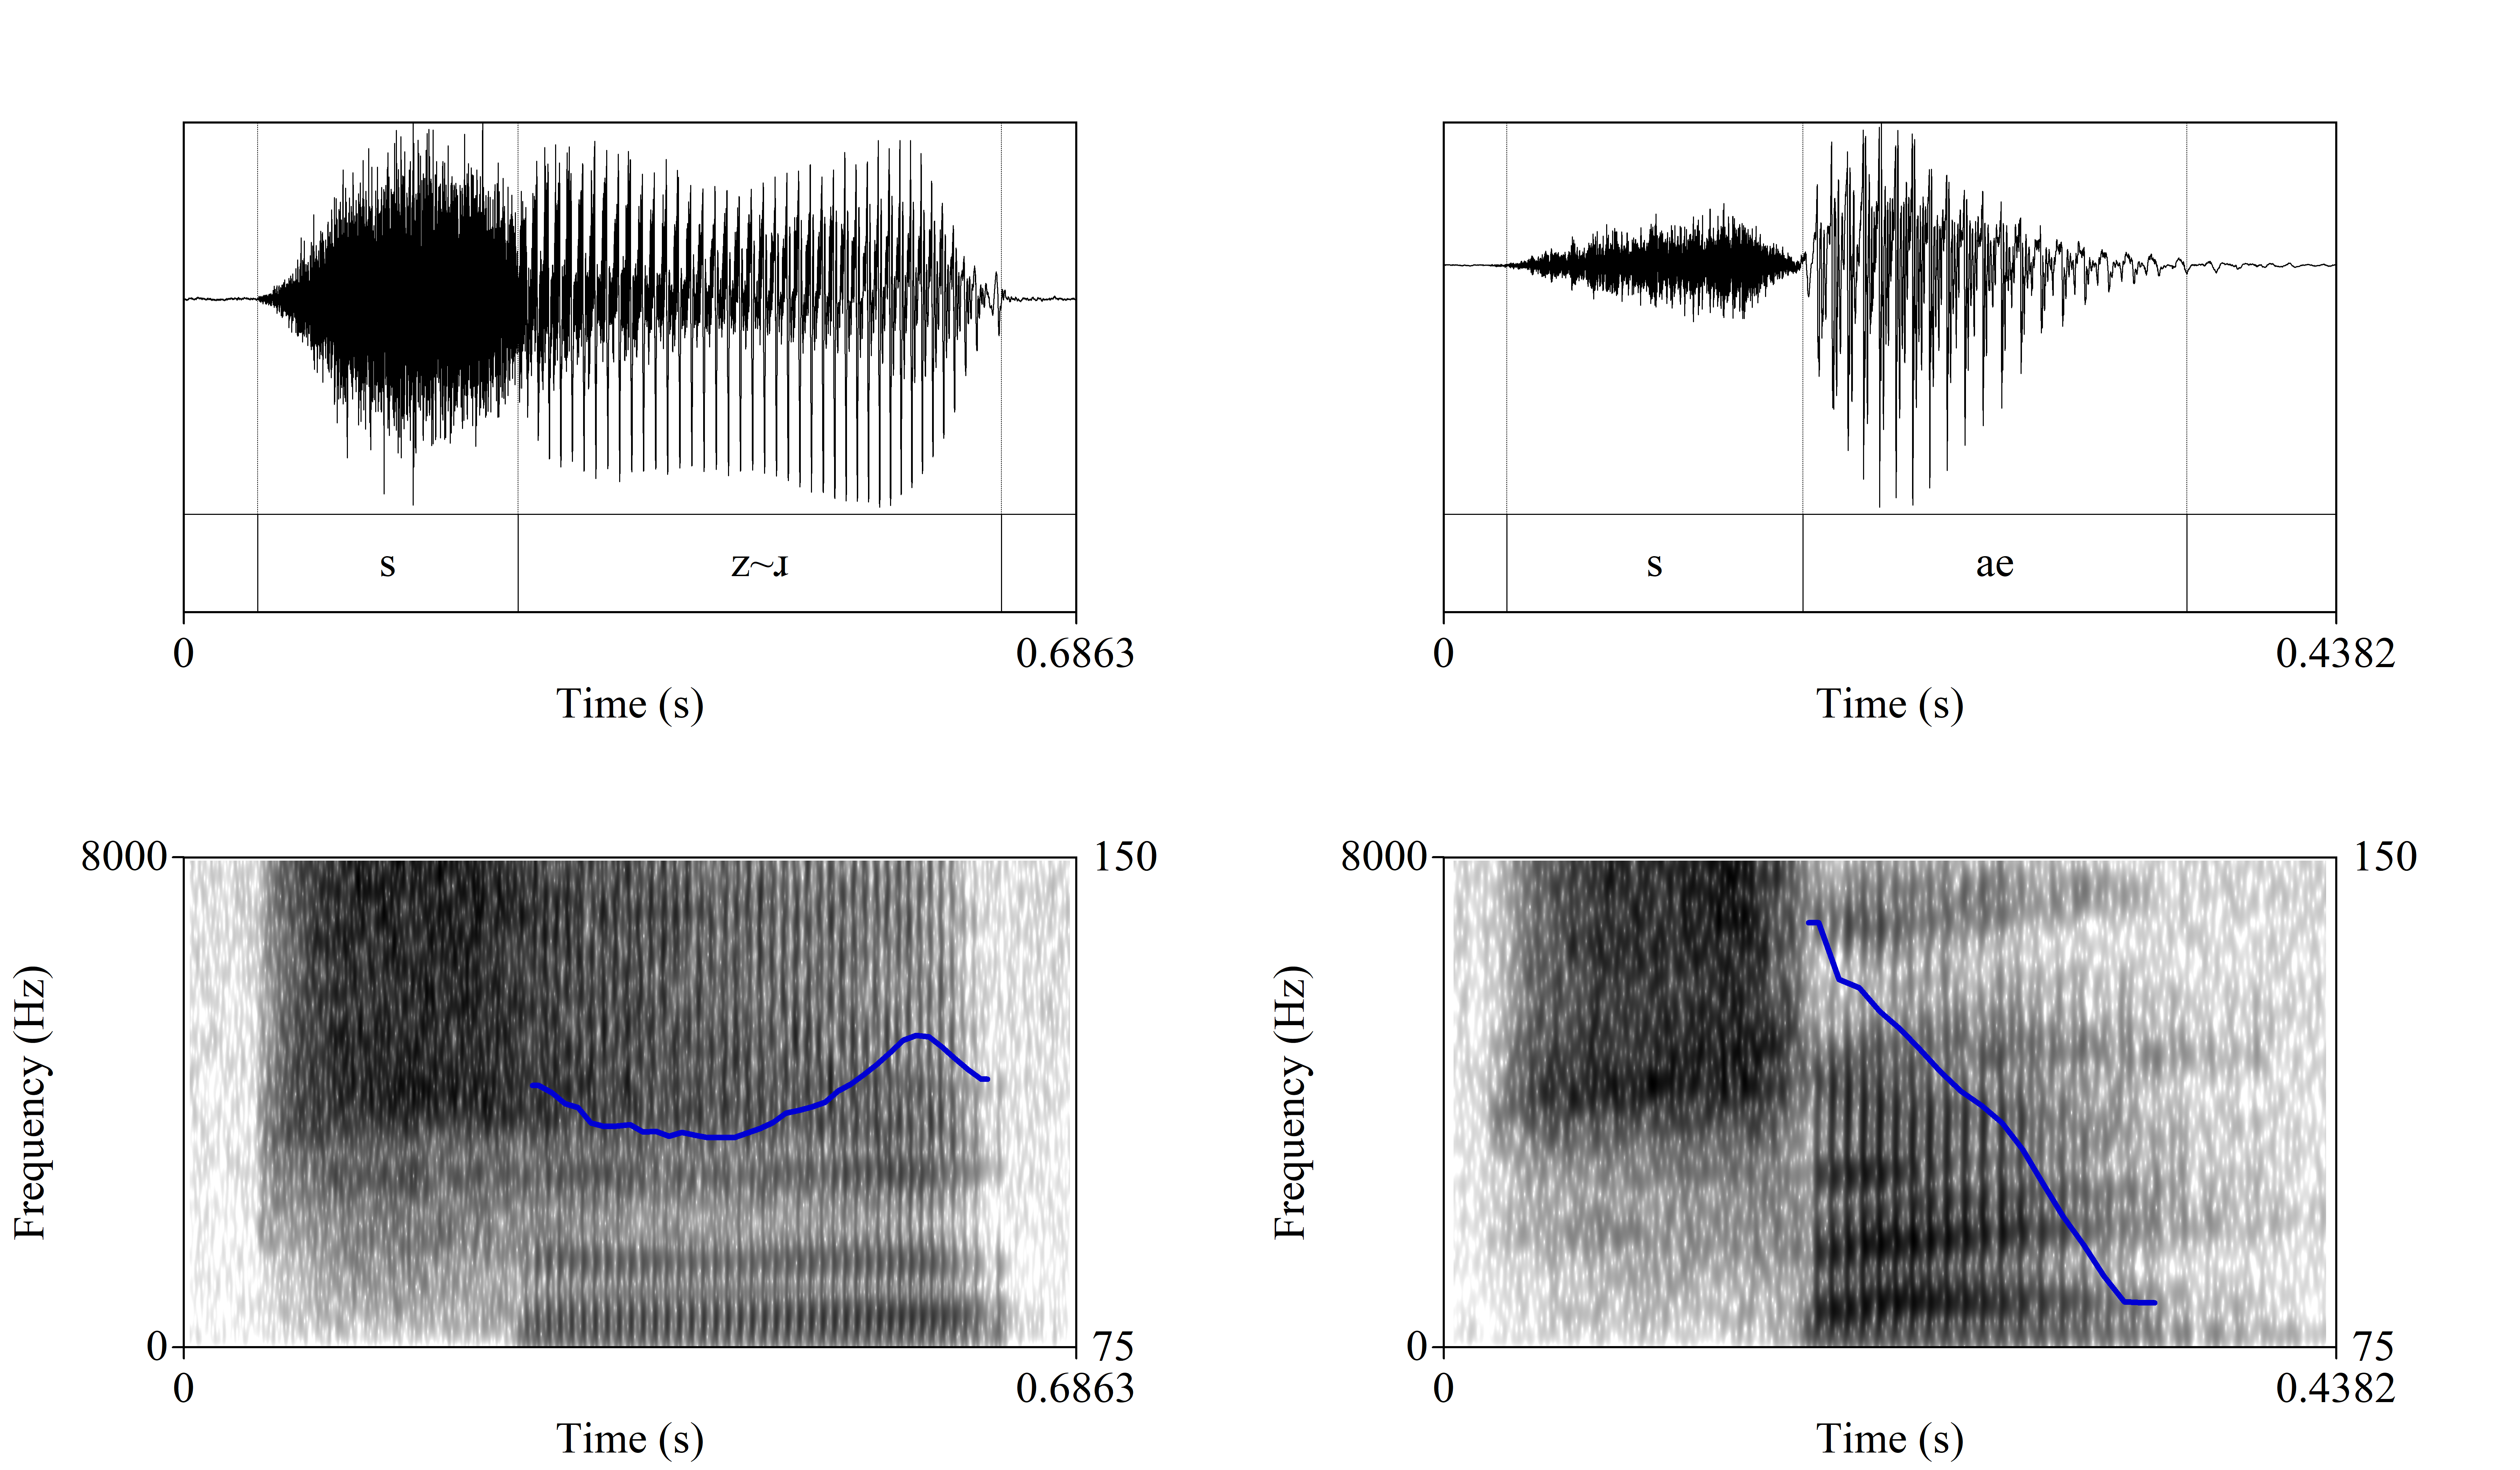
\includegraphics[height=.3\textheight]{figures/FV_example.v5.png}
    \caption{Left: the Zhushan Mandarin word {\cn 死} `to die', which is roughly [sz̩] or [sɹ̩] in standard IPA. Right: the word [sae] {\cn 赛} `race'}
    \label{fig:FV_example}
\end{figure}

The transition from the onset to the nucleus is clearly visible in both spectrograms: the lower formants are well-defined horizontal bands and suggest a sonorant nucleus. However, the higher formants of the nucleus in [sz̩] or [sɹ̩] {\cn 死} `to die' are less discernible because they are masked by the large amount of aperiodic acoustic energy above 4000 Hz. This is audible frication. It is in fact a continuation of the frication of the preceding sibilant onset [s]. Only near the end of the fricative vowel do we see that the frication decreases. This is also visible in the oscillogram, of which the middle portion shows both the regular pulses of a sonorant as well as the jaggedness of a fricative segment. In contrast, the transition from onset to nucleus in [sae] {\cn 赛} `race' shows an immediate drop of energy in higher frequencies, and clear energy concentrations for the vowel formants. This ordinary vocalic nucleus is clearly distinct from the fricative vowel on the left. So what is the precise phonetic and phonological identity of this sound? On the one hand, it is a sonorant nucleus that bears a tone but simultaneously involves frication throughout a significant portion of its realisation. On the other hand, it does not sound like a vowel, it has developed out of a historical *i, and is synchronically still in complementary distribution with Zhushan Mandarin \mbox{/i/}. This illustrates the crux of the matter.

Because of the contradiction between their phonetic and phonological properties, i.e. the combination of their non-vowel-like articulation and obligatory syllabicity, fricative vowels defy a straightforward description with standard terminology and categories. Different lines of research have therefore come to use different terms, analyses, and (IPA) transcriptions that exist alongside each other. This stymies comparative research because it obscures the fact that fricative vowels across different languages have much in common. The general lack of awareness of fricative vowels among linguists maintains the status quo where fricative vowels are typically not included in theoretical discussions and receive little overall attention. The goal of this chapter is therefore to increase the awareness of these intriguing sounds and to point out which important questions they raise.

The structure of this chapter is as follows. Section 2 first provides an overview of different fricative vowels around the world and how they have been transcribed. The section ends with a comparison of the different fricative vowels and a discussion on their ambiguous manner of articulation. Sections 3 and 4 respectively highlight the complexities in their phonetics and phonology. Finally, Section 5 summarises and concludes the chapter.

%%%%%%%%%%%%%%%%%%%%%%%%%%%%%%%%%%%%%%%%%%%%%%%%%%%%%%%%%%%%%%%%%%%%%%%%%%%%%%%%%%%%%%%%%%%%%%%%%%%%%%%%%%%%%%%%%%%%%%%%%%%%%%%%%%%%%%%%%%%%%%%%%%%%%%%%%%%%%%%%%%%%%%%%%%%%%%%%%%%%%%%%%%%%%%%%%%%%%%%%%%%%%%%%%%%%%%%%%%%%%%%%%%%%%%%%%%%%%%%%%%%%%%%%%%%%%%%%%%%%%%%%%%%%%%%%%%%%%%%%%%%%%%%%%%%%%%%%%%%%%%%%%%%%%%%%%%%%%%%%%%%%%%%%%%%%%%%%%%%%%%%%%%%%%%%%%%%%%%%%%%%%%%%%%%%%%%%%%%%%%%%%%%%%%%%%%%%%%%%%%%%%%%%%%%%%%%%%%%%%%%%%%%%%%%%%%%%%%%%%%%%%%%%%%%%%%%%%%%%%%%%%%%%%%%%%%%%%%%%%%%%%%%
\section{Fricative vowels around the world} \label{section2}
All fricative vowels described in this section have certain characteristics in common, but their manner and place of articulation vary. There is thus far no typological framework that categorises them into well-motivated and clearly delineated subgroups, but we will make some preliminary distinctions to add structure to the discussions and to facilitate referring to different fricative vowels. To begin, fricative vowels can be divided into two main groups: those that have labial frication and those that have coronal frication. Among the coronal fricative vowels, it is furthermore useful to separately discuss what we will call the apico-(post)alveolar fricative vowels. This subtype is very common among Chinese (Sinitic) languages, unlike other coronal fricative vowels. For this reason, they are much more extensively researched and are often discussed separately from other coronal fricative vowels. This distinction is sensible for other reasons, too. The apico-(post)alveolar fricative vowels canonically have an apical articulation that sets them phonetically apart from other coronal fricative vowels. In Sinitic languages that have both types of coronal fricative vowels, they can even be phonologically contrastive. The apico-(post)alveolar fricative vowels can also contrast with each other in place of articulation. It is well-established that there is a more anterior one and a more posterior one in Sinitic languages, referred to here as alveolar and postalveolar respectively. The historical origin and synchronic phonological behaviour of these apico-(post)alveolar fricative vowels also differs compared to other coronal fricative vowels. Finally, as will become apparent, there are non-Sinitic languages with fricative vowels that are similar to the apico-(post)alveolar fricative vowels, both phonetically and phonologically. It thus seems useful to distinguish them as a subtype of coronal fricative vowels beyond Sinitic languages. We emphasise, however, that this coronal subgrouping must not be understood as a simple division based on the passive or active articulators. Instead, this division takes all factors mentioned above into account, including historical origin. What this means is that this division does not preclude any coronal fricative vowel from being postalveolar or apical, even if it is not considered as belonging to the apico-(post)alveolar subtype.


\largerpage
It is worth noting that making a distinction of fricative vowels based on manner of articulation is not straightforward either. This issue is highly controversial and, as an inevitable consequence, there are also many discrepancies in terminology and transcription. As stated, we adopt the term ``fricative vowel" from \citet{Ladefoged&Maddieson_1996} here because it is the most widely known term. However, fricative vowels have also been referred to as ``apical vowels" \citep{Karlgren_1915}, ``apical dorsal vocoids" \citep{Demolin_2002}, ``obstruent vowels" \citep{Faytak_2014a}, ``strident vowels" \citep{Hu&Ling_2019}, ``syllabic fricatives" (\cite[47]{Chao_1968}; \cite[44]{Duanmu_2007}; \cite[72]{Lin_2007}; \cite{Chen&Gussenhoven_2015}; \cite{shao_2020}), ``syllabic approximants" (\cite{Lee&Zee_2003}; \cite{Chen&Guo_2022}), ``extra high vowels" \citep{Yoder_2020}, ``laminal vowels" \citep{Aoi&Niigata_2013}, and ``coronal vowels" or ``blade vowels" \citep{laver_1994}.

In this section, we begin the global overview of fricative vowels with Sinitic languages because they contain the most well-described and most diverse fricative vowels. Apico-(post)alveolar (§\ref{section:alv_postalv_FVs}), other coronal (§\ref{othercoronal}), and labial (§\ref{labial.fvs}) fricative vowels are all attested in Sinitic languages, and some regional varieties even have all three. Each type could be further divided based on more precise places of articulation as well as the presence or absence of lip rounding. Section §\ref{non-sinitic} discusses fricative vowels in other languages.

%%%%%%%%%%%%%%%%%%%%%%%%%%%%%%%%%%%%%%%%%%%%%%%%%%%%%%%%%%%%%%%%%%%%%%%%%%%%%%%%%%%%%%%%%%%%%%%%%%%%%%%%%%%%%%%%%%%%%%%%%%%%%%%%%%%%%%%%%%%%%%%%%%%%%%%%%%%%%%%%%%%%%%%%%%%%%%%%%%%%%%%%%%%%%%%%%%%%%%%%%%%%%%%%%%%%%%%%%%%%%%%%%%%%%%%%%%%%%%%%%%%

\subsection{Fricative vowels in Sinitic languages} \label{sectionsinitic}
\subsubsection{Sinitic-type apico-(post)alveolar fricative vowels} \label{section:alv_postalv_FVs}
The apico-(post)alveolar fricative vowels are by far the most extensively studied owing to their widespread occurrence across almost all branches of the Sinitic family \citep{Cui_2021}, as well as the fact that this type appears in Standard Mandarin Chinese. As such, discussions on manner of articulation, terminology, and transcription have mostly focused on apico-(post)alveolar fricative vowels. They are typically called ``apical vowels" in the literature, but they have also been analysed as fricatives and approximants, as discussed below. Canonically, their articulation is described as involving a raised tongue tip similar in position to sibilants. The example of a fricative vowel given above in \figref{fig:FV_example} is of this type. Below in (\ref{FV_examples_HEFEI}) there are more examples from Hefei Mandarin, which has three of such fricative vowels. In these phonemic transcriptions from \citet{Kong_et_al_2022}, the fricative vowels are transcribed with approximant symbols and the numerals indicate tonal levels. There are two alveolar fricative vowels, an unrounded (\ref{FV_examples_HEFEI}a-b) and a rounded one (\ref{FV_examples_HEFEI}c), as well as an unrounded postalveolar fricative vowel (\ref{FV_examples_HEFEI}d-e).

\ea \label{FV_examples_HEFEI}
    \begin{tabbing}
        \quad \=a. \quad \=sɹ\textsuperscript{53} \qquad \={\cn 事} `thing' \qquad \qquad \qquad \=d.\quad\= ʃɻ\textsuperscript{24} \quad \= {\cn 时} `time' \\
        \>b.\> pɹ\textsuperscript{213} \> {\cn 比} `to compare' \>e.\> tʃɻ\textsuperscript{213} \> {\cn 纸} `paper'\\
        \>c. \>zɹ\textsuperscript{w 213} \> {\cn 雨} `rain'
    \end{tabbing}
\z

Traditionally, apico-(post)alveolar fricative vowels have been treated as vowels within modern Chinese linguistics. Historically, their general source is high front vowels, which can still be found in cognates of sister languages without fricative vowels. For example, Hefei Mandarin /sɹ\textsuperscript{53}/ `thing' corresponds to /si\textsuperscript{22}/ in Hong Kong Cantonese. Furthermore, ancient philologists of the first and second millennia made no distinction between rhymes with vowels and rhymes with fricative vowels in their classifications of syllables \citep{shen_phonological_2020}. However, this does not necessarily mean that they considered fricative vowels to have the same manner of articulation as regular vowels. After all, philologists were not concerned with manner of articulation in the modern linguistic sense and instead sought to efficiently order the logographic writing system of Chinese characters in dictionaries. Categorising fricative vowels along with other rhymes is convenient for classification given that a distinction between vocalic rhymes and non-vocalic rhymes is superfluous. Alternatively, this philological convention may well predate the emergence of fricative vowels in Sinitic languages, so the categorisation of fricative vowels as vowels by later philologists may merely reflect a continuation of tradition and not a contemporary phonetic/phonological analysis. Regardless, the vowel-analysis of apico-(post)alveolar fricative vowels is still influential among Chinese linguists. It is also warranted on the grounds of complementary distribution: the apico-(post)alveolar fricative vowels are often in complementary distribution with each other and with /i/. This is the case for Mandarin varieties such as Hefei Mandarin \citep{Kong_et_al_2022} shown above and for Standard Chinese,\footnote{The
    single, possible exception to this complementarity could be {\cn 日} [ɻ̩] 'sun, day' if one analyses it as /ɻ̩/ instead of /ɻɻ̩/. It would then form a minimal pair with e.g. {\cn 易} 'easy' /i/.
}
and sometimes also applies to non-Mandarin varieties such as Shanghai Wu \citep{Chen&Gussenhoven_2015} and Xiangxiang Xiang \citep{Zeng_2020}. On the other hand, there are many languages in which fricative vowels \textit{do} contrast with /i/, such as Suzhou Wu \citep{Hu&Ling_2019}, Meixian Hakka \citep{Lee&Zee_2009}, and Yichun Gan \citep{Li_2018}. However, when there is a complementary distribution, the apico-(post)alveolar fricative vowels can often be analysed as allophones of /i/, albeit with a very different realisation. The conditioning environment for the allophony is then the onset, which is very often phonotactically restricted to sibilant fricatives or affricates. Additional arguments in support of the vowel-analysis are given by \citet{baron_1974}. He lists fricative vowels' long duration compared to consonants, their ability to bear tone, and their capacity to be in the syllable nucleus. These three arguments, however, cannot be considered as independent because they are all general properties of nuclei in Sinitic languages. Most of the arguments for a vowel-analysis are phonological in nature rather than phonetic. When considering articulation and acoustics, there are fewer favourable arguments available. One argument is that the fricative vowels have a clear formant structure \citep[10]{Howie_1976}, which is commonly considered an important property of vowels and not of fricatives. It was probably for the reasons above that the first linguist to describe the apico-(post)alveolar fricative vowels, \citet{Karlgren_1915}, chose to analyse them as vowels. He coined the term ``apical vowels" and invented the symbols /ɿ, ʅ, ʮ, ʯ/ to transcribe them. The symbols /ɿ/ and /ʅ/ are respectively alveolar and postalveolar, and /ʮ/ and /ʯ/ are their rounded counterparts. These symbols are widely used among Chinese dialectologists but are not officially recognised by the IPA.

An opposing view is that the apico-(post)alveolar fricative vowels are fricatives. Instead of needing to invent new symbols, proponents of this analysis use the standardised IPA symbols /z, ʐ, zʷ, ʐʷ/ to indicate that the pronunciation is roughly that of a voiced sibilant.\footnote{Some of the sources mentioned here actually only provide IPA transcriptions for the \textit{unrounded} apico-(post)alveolar fricative vowels because the sound systems described in them only have unrounded fricative vowels. However, one can extrapolate from the symbols for unrounded fricative vowels that these authors might use the same symbols with the superscript [ʷ] to indicate roundedness, as \citet{Kong_et_al_2022} did in their description of Hefei Mandarin. It should furthermore be noted that the retroflexion in phonetic symbols such as /ʐ, ʅ, ʯ/ for the postalveolar fricative vowels does not suggest an articulation with the tongue tip curled backwards, but instead an apical postalveolar sound, as is the convention within the literature.} \citet{Duanmu_2007}, \citet{Lin_2007}, and \citet{Wiedenhof_2015} consider them to be syllabic fricatives in Standard Chinese. However, Duanmu and Lin assume that this is only the case at the phonetic level, as will be discussed in Section 4. The reasons for a fricative-analysis of apico-(post)alveolar fricative vowels are very straightforward. First, there may be so much constriction that strong frication is involved, which is simply not characteristic for vowels. Second, their articulation is often assumed to differ only minimally from the sibilant onsets that typically obligatorily precede them. This gives the impression that the only difference between the sibilant onset and the fricative vowel nucleus is voicing. That is, the fricative vowel is a voiced fricative. This assumption has been verified for some Sinitic varieties by articulatory research. \citet{Lee-Kim_2014} and \citet{faytak&lin_2015} showed that there is generally little change in tongue position in Standard Chinese between the sibilant onset and nucleus for apico-postalveolar fricative vowels. \citet{shao_2020} found the same result for the Jixi Hui apico-alveolar fricative vowel and also examined its acoustic characteristics. Based on both articulatory and acoustic evidence, he adopts the fricative-analysis for Jixi Hui.

\largerpage
A third view is that apico-(post)alveolar fricative vowels are best analysed as approximants (\cite{Lee&Zee_2003}; \cite{Lee-Kim_2014}; \cite{Li&Zhang_2017}; \cite{Huang&al_2021}; \cite{Kong_et_al_2022}). Those who prefer an approximant-analysis may use the standard symbols /ɹ̺, ɻ, ɹ̺ʷ, ɻʷ/. The diacritic [\textcolor{white}{X}̺] for apical articulation in the alveolar sounds is often omitted for convenience. What makes this analysis appealing is that apico-(post)alveolar fricative vowels do not always involve strong frication. \citet{faytak&lin_2015} even report that some speakers employ an articulatory strategy that actively decreases frication. When frication \textit{is} produced, it may merely be a carryover effect from the preceding sibilant \citep[274]{Lee-Kim_2014}. Another argument is that the first and second formants of apico-(post)alveolar fricative vowels do not respectively correspond to the size of the pharyngeal and oral cavities as resonance chambers, as is the case in normal vowels (\cite{Ling_2007}; \cite{Ling_2009}; \cite{Lee-Kim_2014}). This means that the formants cannot be interpreted as indications of backness and openness. As a result, the positions of the apico-alveolar and apico-postalveolar fricative vowels within a vowel chart do not make sense relative to each other or to the positions of regular vowels. The position of apico-alveolar fricative vowels is more back in the chart than that of apico-postalveolar ones, which is misleading. Lee-Kim argued that these acoustic findings are more consistent with an analysis of these sounds as consonants. The arguments in favour and against each of the three analyses are summarised in \tabref{tab:arguments}.

\begin{table}
    \caption{A summary of the arguments for each analysis of the apico-(post)alveolar fricative vowels in Sinitic languages. A ``+" indicates that the argument supports the analysis, a ``-" indicates a weakness, and ``+/-" indicates that the argument neither supports nor weakens the analysis}
\label{tab:arguments}
 \begin{tabularx}{\textwidth}{Q cccc}
  \lsptoprule
     & as vowels & as fricatives & as approximants \\
    & /ɿ, ʅ, ʮ, ʯ/ & /z, ʐ, zʷ, ʐʷ/ & /ɹ̺, ɻ, ɹ̺ʷ, ɻʷ/ \\
  \midrule
complementary with /i/ & + & - & - \\
\tablevspace
tone, duration, nuclear position & + & - & +/-\\
\tablevspace
formant structure & + & +/- & + \\
\tablevspace
variable frication & - & - & +/- \\
\tablevspace
acoustics of F1 and F2 & - & + & + \\
\tablevspace
articulatory overlap with sibilants & - & + & - \\
  \lspbottomrule
 \end{tabularx}
\end{table}

\newpage
As could be expected, the arguments in favour of the vowel-analysis do not support a fricative-analysis and vice versa, and the approximant-analysis takes an intermediate position. Complementary distribution of apico-(post)alveolar fricative vowels with /i/ in Sinitic languages is common, and, when it applies, it is a valid argument for an analysis as (underlying) vowels. However, general nuclear properties such as bearing tone are not compelling. Syllabic consonants can also bear tone, have long duration and are by definition nuclear. Similarly, visible formant structures are not exclusive to vowels either \citep[35]{Duanmu_2007}. The argument of frication is, in fact, a problem for all analyses because the frication is not consistently there. Its variable presence is nevertheless the least inconsistent with the approximant-analysis. Finally, the formant values and the articulatory gesture support a consonantal analysis. Considering all the arguments, it should not be surprising that the debate on manner of articulation has gone on for decades. No consensus has been reached on the optimal analysis for Standard Chinese, let alone a uniform analysis for all Sinitic languages.

\subsubsection{Other coronal fricative vowels} \label{othercoronal}
Other coronal fricative vowels typically involve a raised tongue blade that creates frication through its close proximity to the palate, although there are also speakers who pronounce them with an apical gesture (\cite{Ling_2009}; \cite{Faytak_2022}). Like their apico-(post)alveolar counterparts, the predominantly laminal coronal vowels have cognates with high vowels in related varieties that do not have these fricative vowels. What sets them apart from the apico-(post)alveolar sounds, however, are their free phonotactics and their more sparse geographical distribution. These coronal fricative vowels do not occur in Standard Chinese and are known to occur mostly in Wu Chinese \citep{Faytak_2018}, the Jianghuai Mandarin group \citep{Shi_1998}, and Jin Chinese \citep{Karlgren_1915}. The following Suzhou Wu examples show (near-)minimal pairs between regular vowels and two coronal fricative vowels \citep[73]{Faytak_2018}, with the fricative vowels on the right. The symbols /i͡ʑ/ and /y͡ʑ/ are digraphs for unrounded and rounded fricative vowels, respectively.

\ea \label{data_Suzhou}
    \begin{tabbing}
        \quad \= i\textsuperscript{44} \quad \={\cn 烟} `smoke' \qquad \quad\= i͡ʑ\textsuperscript{44} \quad \={\cn ⾐} `clothes' \\
        \>si\textsuperscript{44} \>{\cn 鲜} `fresh' \> si͡ʑ\textsuperscript{44} \>{\cn 西} `west'\\        
        \>y\textsuperscript{523} \>{\cn 怨} `blame' \> y͡ʑ\textsuperscript{44} \>{\cn 迂} `circuitous'\\
        \> ɕy\textsuperscript{44} \>{\cn 休} `rest' \> ɕy͡ʑ\textsuperscript{44} \> {\cn 虚} `weak'
    \end{tabbing}
\z

This type of coronal fricative vowels is referred to in the literature with the general terms ``strident vowels" and ``fricative vowels" (\cite{Ladefoged&Maddieson_1990}; \cite{Hu&Ling_2019}). However, within Chinese linguistics in particular, ``fricative vowel" is sometimes used in a narrow sense that explicitly does \textit{not} include the apico-(post)alveolar type (\cite{Ling_2007}; \cite{Hu&Ling_2019}; \cite{Faytak_2022}). In such cases, it is a translation of the term \textit{mócā huà yuányīn} {\cn 摩擦化元音} `fricativised vowel', as opposed to \textit{shéjiān yuányīn} {\cn 舌尖元音} `apical vowel'. The non-apical coronal fricative vowels always involve frication but are nonetheless invariably analysed as vowels within Chinese linguistics.

There appear to be only two types of these coronal fricative vowels in Sinitic languages: the unrounded variant and the more rare rounded variant, both of which are given in (\ref{data_Suzhou}). Nevertheless, many transcriptions are in use because there is even less standardisation than for the apico-(post)alveolar fricative vowels. Because there is no official diacritic for frication in the IPA, there are authors who use sub- or superscript fricatives next to high vowels, e.g. [i\textsubscript{z}], [i\textsuperscript{z}], or  [i\textsubscript{ʑ}, y\textsubscript{ʑ}] (\cite{Ling_2007}; \cite{Faytak_2019}). \citet{Wu_2013} suggests [i\textsubscript{j}, j, ʑ] for unrounded coronal fricative vowels of various levels of frication, with a subscript \textsubscript{j} instead.\footnote{The transcription [ʑ] for the most fricated coronal fricative vowels does seem to indicate that \citet{Wu_2013} considers some realisations to be fricatives, but his work is not concerned with the phonological implications.} The IPA diacritic for extra close articulation is also sometimes used, i.e. [i̝, y̝] \citep{Hu&Ling_2019}. Another IPA alternative without diacritics would be [ʝ, ʝʷ]. Recently, \citet{VandeWeijer&al_2021} and \citet{Shi&Chen_2022} opted for transcriptions such as \mbox{[i̟ ,} y̟] in Wu Chinese to indicate that the articulation of these segments is more fronted than that of regular front vowels.

\subsubsection{Labial fricative vowels} \label{labial.fvs}
Finally, there are fricative vowels that have a labial constriction, be it bilabial or labiodental. Some also have an additional dorsal constriction (\cite{Hu&He_2019}; \cite[48]{shao_2020}). According to \citet[258]{Pan_1991}, the unrounding of /u/ to a segment with compressed lips is a characteristic of Wu, Gan, Hakka, and Min Chinese. In at least some cases, such segments have developed into fricative vowels. Labial fricative vowels are generally rare in Mandarin, but they do occur in more western Mandarin varieties, such as in Guanzhong \citep{Zhang_and_Xing_2011} and Xining \citep{Dede_2006}. Below are some Xining Mandarin examples adapted from \citet[324]{Dede_2006}.

\ea \label{data_xining}
    \begin{tabbing}
        \quad \= lv\textsuperscript{22} \quad \={\cn 路} `road'\\
        \>lv\textsuperscript{35} \>{\cn 炉} `stove' \\
        \> tʃv\textsuperscript{55} \>{\cn 猪} `pig' \\
       \> v\textsuperscript{53} \>{\cn 五} `five'
    \end{tabbing}
\z

Labial fricative vowels are also referred to as ``fricative vowels" in a narrow sense that excludes the apico-(post)alveolar type, and some of them have been referred to as ``labiodental vowels" \citep{Hu&He_2019}. Phonological transcriptions typically use vowel symbols, although the corresponding realisations may be transcribed with consonantal symbols (\cite{Hu&He_2019}; \cite{Yuan&al_2019}). 

Various kinds of labial fricative vowels have been attested. Some have a labiodental constriction, as the data in (\ref{data_xining}) show. Others have a bilabial constriction \citep{Faytak_et_al_2019}. Furthermore, in some varieties of Sinitic, the tongue dorsum simultaneously adds a front vowel or back vowel quality (\cite{Hu&He_2019}; \cite[48]{shao_2020}), while this is not the case in other varieties \citep{Faytak_et_al_2019}. Assuming these parameters of labial constriction (bilabial/labiodental) and lingual constriction (front/back/absent), one could distinguish as many as six different types of labial fricative vowels based on place of articulation. Given the above, it should not be surprising that there are once again many different transcriptions in use. The phonological transcription is usually /u/ unless the labial fricative vowel(s) contrast with a regular non-fricated vowel /u/, although /ɯ/ may be used instead to express the fricative vowel's lack of rounding. The labial constriction can be phonetically transcribed with common IPA symbols [v̩ , ʋ̩] for labiodental fricative vowels (\cite{Zhang_and_Xing_2011}; \cite{Scholz_2012}; \cite{Hu&Ling_2019}), and, although we have not encountered this transcription, [β̩ ] could theoretically be used for bilabial fricative vowels. Alternatively, superscript or subscript are used, such as [u\textsubscript{β}, ɯ\textsuperscript{β}, ɯ\textsuperscript{v}] (\cite{Zhu_2004}; \cite{Faytak_et_al_2019}). The presence or absence of a dorsal constriction may be difficult to ascertain without articulatory research, and it is typically not mentioned in descriptions. An exception is a study by \citet{Hu&He_2019}, who characterise the constriction of the two labial fricative vowels in Rui'an Wu as a labiodental constriction superimposed on a front vowel [y] and a back vowel [u]. Because these sounds contrast in backness, the authors use the non-fricative vowel symbols /ʉ/ and /ɯ/. For Jixi Hui, \citet[48]{shao_2020} proposes a narrow transcription [v̩ˠ] to indicate the ``highly velarised" allophone of /u/ when it follows labiodental onsets.

%%%%%%%%%%%%%%%%%%%%%%%%%%%%%%%%%%%%%%%%%%%%%%%%%%%%%%%%%%%%%%%%%%%%%%%%%%%%%%%%%%%%%%%%%%%%%%%%%%%%%%%%%%%%%%%%%%%%%%%%%%%%%%%%%%%%%%%%%%%%%%%%%%%%%%%%%%%%%%%%%%%%%%%%%%%%%%%%%%%%%%%%%%%%%%%%%%%%%%%%%%%%%%%%%%%%%%%%%%%%%%%%%%%%%%%%%%%%%%%%%%%

\subsection{Fricative vowels elsewhere} \label{non-sinitic}
Compared to the fricative vowels in Sinitic languages, those in other language families are less abundantly attested. However, it is still clear that fricative vowels can be found in many geographically non-contiguous regions, and all subtypes of fricative vowels as described in §\ref{sectionsinitic} can be identified in non-Sinitic languages, too. A selection of diverse and representative languages is discussed per region.

\subsubsection{Ryukyuan islands}
Fricative vowels have been reported in Japonic languages spoken in the Ryukyu archipelago south of mainland Japan. Some Southern Ryukyuan languages such as Miyako have a fricative vowel where related varieties have /i/ or /ɨ/ \citep{Jarosz_2018}, which is reminiscent of the situation for Sinitic apico-(post)alveolar fricative vowels. The Ryukyuan segment has been called ``fricative vowel" by some \citep{Pellard&Hayashi_2012} but has also been referred to as an ``apical vowel" \citep{Jarosz_2018} or ``laminal vowel" \citep{Aoi&Niigata_2013}. \citet{Jarosz_2018} and \citet{Pellard&Hayashi_2012} use the symbol /ɿ/, deliberately choosing the same non-standard symbol that is used for the apico-alveolar fricative vowel in Chinese linguistics. Although most researchers in this field consider the Ryukyuan fricative vowel to be a vowel, \citet[15]{Pellard&Hayashi_2012} mention that at least some researchers describe the fricative vowel as a consonant. For example, \citet{Sawaki_2000} notes that native speakers of Miyako accept a pronunciation of [z] as correct. He also writes that this segment sounds like [s] when it is devoiced (devoicing is common and predictable for high nuclei in Japonic languages). The phonotactics of the fricative vowel vary: this sound occurs after various labial and coronal onsets in Irabu Miyako, but is restricted to homorganic sibilant onsets in Ikema Miyako \citep{Pellard&Hayashi_2012}. Unlike the apico-alveolar sounds in Sinitic languages, however, the Ikema Miyako fricative vowel reportedly used to have a wider distribution until it merged with *i in all cases except for after the sibilant onsets \citep[16]{Pellard&Hayashi_2012}. Finally, it is unclear whether the syllabic [v̩] in some Ryukyuan languages is a labial fricative vowel, because it is not referred to as a vowel by any of the sources cited here. It has cognates with /u/, and its historical development parallels that of the Ryukyuan sound that \textit{is} considered to be a fricative vowel \citep{Jarosz_2018}.

\subsubsection{Africa}
Fricative vowels in Africa have been attested in and around Cameroon in most branches of the Bantoid language family, a subgroup within the larger Atlantic-Congo family. They occur in Mambila \citep{connell_2007}, Grassfields languages such as Limbum (\cite{Fransen_1995}; \cite{Faytak_2017}) and Kejom \citep{Faytak&Akumbu_2021}, Beboid languages such as Nchane \citep{boutwell_2020}, Yemne-Kimbi languages such as Mundabli \citep{Voll_2017}, and at least in one Bantu language called Fang \citep{Kelly_1974}. All these Bantoid languages are (distantly) related, so it may be difficult to disentangle inherited traits from borrowed ones. It should be noted that a pair of ``extra high vowels" *i and *u, distinct from regular *i and *u, is reconstructed for Proto-Bantu. The extra high vowels conditioned spirantisation of preceding onsets in several Bantu languages, and some authors have proposed that these vowels could have been phonetically similar to some present-day fricative vowels (\cite{connell_2007}; \cite{Faytak_and_Merrill_2014}).

Judging by the transcriptions used for fricative vowels in central Western Africa, these languages have coronal and labial fricative vowels. For the coronal group, one can find phonetic transcriptions such as [i̻ , ʑ͜i, z̩ , ʒ̩]. For example, the digraph [ʑ͜i] is used to transcribe the fricative vowel in Fang \citep{Kelly_1974}, which has a free phonotactic distribution and is a full-fledged phoneme. In Kejom, on the other hand, the coronal fricative vowel transcribed as [i̻] occurs only as an allophone of /i/ after postalveolar sibilants \citep{Faytak&Akumbu_2021}. Kejom also has a rounded coronal fricative vowel [ʉ̻] as an allophone of /ʉ/, which similarly only occurs after postalveolar sibilants. All in all, the Fang and Kejom fricative vowels appear to differ considerably in terms of their phonetics and phonology. The labial fricative vowels in this area are equally diverse. One can find at least [v͜ɯ, ʉ\textsuperscript{v}, ʉ\textsuperscript{β}, v̩] as transcriptions. Some sounds, such as Kejom /ʉ\textsuperscript{v}/ and /ʉ\textsuperscript{β}/, are predictable and only appear after homorganic onsets, while Limbum [v̩] and Mambila [v͜ɯ] can co-occur with multiple onsets. Sometimes authors use plain [i, ɨ, u, ʉ] with the verbal description of ``fricated", as \citet{Voll_2017} does for Mundabli and \citet{boutwell_2020} for Nchane. Based on the information above, one can generalise that fricative symbols are used for fricative vowels with a free distribution and that vocalic symbols are used for fricative vowels with a restricted distribution. However, none of the authors cited here consider the fricative vowels to be consonants at the underlying level.

An African language with fricative vowels that is geographically and genetically unrelated to those mentioned above is Lendu, a Central Sudanic language, which is spoken in the Democratic Republic of the Congo. \citet{Kutsch_Lojenga_1989} writes that Lendu has two contrastive fricative vowels, both of which are realised roughly as [z̩]. Kutsch Lojenga describes one as ``sharp" and the other as ``dull", and explains that there is a difference in voice quality that cannot be captured with IPA symbols. She indicates the difference by adding a `` ˈ " symbol after the sharp fricative vowel, and  ``*" after the dull one. The following data are adapted from \citet[120]{Kutsch_Lojenga_1989}.\footnote{On the cited page, Kutsch Lojenga uses transcriptions that are neither phonetic nor phonological (she adjusts them at a later stage in her argumentation). For both fricative vowels, she uses ``s" for [z̩] when preceded by a voiceless sound, and ``z" for [z̩] when preceded by a voiced onset. Here, both are transcribed as [z̩], followed by ˈ or *.}
\newpage

\ea \label{Lendu_data}
    \begin{tabbing}
        \quad \= [ɪ̀.sz̩̄]ˈ \quad \= `woman' \qquad \qquad \= [sz̩̄]* \quad \= `shoe'\\
        \>[tsž̩]ˈ\>`red kaolin' \>[tsž̩]*\> `lawn'\\
        \>[zz̩̄]ˈ \>`brother-in-law' \> [zz̩̄]* \> `to milk (a cow)'\\
        \>[dzz̩̀]ˈ\>`price'\>[dzz̩̀]*\>`to weep'
    \end{tabbing}
\z

Both fricative vowels can only follow alveolar sibilants /s, z, ts, dz/. If the onset is voiceless, there is a slight non-contrastive delay in voicing in the transition from the onset to the fricative vowel nucleus. This limited phonotactic distribution and the phonetic descriptions of the Lendu fricative vowels are similar to what is common for the Sinitic apico-alveolar fricative vowels. There is also phonetic data on Lendu. \citet{Demolin_2002} reanalysed the Lendu syllabic [z̩] as a vowel based on data from acoustics, aerodynamic measures, electroglottography, and visual recordings of jaw movements.\footnote{Curiously, Demolin mentions nothing of the ``sharp/dull" distinction made by \citet{Kutsch_Lojenga_1989}. The latter cites other, older sources in her paper that make a similar distinction: ``\citet[30]{Tucker_and_Bryan_1966} refer to this particular contrast as ``dark" as opposed to ``clear" articulation ... though their examples are not completely consistent with my data" (\citeyear[120]{Kutsch_Lojenga_1989}). The situation is therefore unclear.} According to Demolin, there is articulatory overlap between sibilant onsets and the syllabic segments that follow. This articulatory overlap causes the frication during the syllable nucleus, which is why this sound has been perceived as a fricative by linguists working on Lendu. Demolin furthermore compares the spectral properties of Lendu fricative onsets, fricative vowels, and regular vowels. The data show that the fricative vowels have visible formant structures and less intense frication than fricatives in the onset. Recall that the Zhushan Mandarin example in \figref{fig:FV_example} can be characterised in the same way and is likewise restricted to having homorganic sibilant onsets. As such, both the phonotactic distribution and the phonetic properties of the Lendu fricative vowels are comparable to the Sinitic apico-alveolar vowels.

\subsubsection{New Guinea}
A number of Lakes Plain languages on the island of New Guinea (the Indonesian half) have coronal fricative vowels. A front unrounded one and a back rounded one have been attested, respectively transcribed as [i', u'] \citep{Foley_2018} or [i̝ , u̝] \citep{clouse&clouse_1993}. Some languages, such as Iau and Abawiri \citep{Yoder_2020}, only have the unrounded fricative vowel, while others, such as Doutai and Kirikiri \citep[533]{Foley_2018}, have both. None have only a rounded fricative vowel. The fricative vowels in Lakes Plain languages are always considered to be vowels. However, there is reason to believe that the Papuan fricative vowels do not have a high degree of frication compared to those elsewhere. Consonantal transcriptions such as [ʑ] have not been used in the Papuan literature, and Yoder explicitly describes the frication in Abawiri as only ``faintly audible" (\citeyear[57]{Yoder_2020}).

\subsubsection{Europe}
In some varieties of Swedish, one can find the so-called Viby-\textit{i} and Viby-\textit{y}, named after the Swedish village of Viby. The vernacular pronunciation of the village name has both of these sounds. They are the realisations of /iː, yː/ that have a distinctive ``damped" character and which reportedly often involve frication (\cite{Björsten&Engstrand_1999}; \cite{Grönberg_2004}). For speakers that have the Viby-\textit{i} and Viby-\textit{y}, those realisations have replaced ordinary [iː] and [yː]. \citet{westerberg_2020} provides an in-depth phonetic study of these sounds. She writes that although they are not the standardised pronunciations, they are extremely common in Sweden's largest cities and sometimes considered as posh. Less common are ``Viby-coloured" short /ɪ, ʏ/, but they are attested in e.g. the Bohuslän dialect \citep[70]{westerberg_2020}. \citet[53]{westerberg_2020} lists the following transcriptions for Viby-\textit{i} in the literature: [iː\textsuperscript{z}, ɨ, ð, ʅ]. There are fewer descriptions of the Viby-\textit{y}. \citet{Björsten&Engstrand_1999} consider the contrast between /iː/ and /yː/ to be neutralised, and \citet{Gross&Forsberg_2020} confirm that there is perceptual overlap. However, \citet[194]{westerberg_2020} shows that a visible difference in lip posture is still present between /iː/ and /yː/.

\subsubsection{Central and East Asia (non-Sinitic)}
Although fricative vowels are best-studied in the Sinitic language family, they are an areal phenomenon in other languages of the region as well. They often occur in Tibeto-Burmese languages, which are only distantly related to Sinitic. An example is Nuosu Yi, as described by \citet{Edmondson&al_2017}, a Lolo-Burmese language spoken in Southern China. It has two pairs of fricative vowels: /z, z̠/ and /u, u̠/, where the retractedness in the phonemic notation is realised as a retracted tongue root and the labial fricative vowels are actually realised as [v] with a vowel offglide. Therefore, \citet{Edmondson&al_2017} transcribe the realisations as [z, z̙ , vʊ, vɵ̙]. The alveolar pair also has retroflex allophones [ʐ, ʐ̙] after retroflex onsets. As indicated by the transcriptions, \citet{Edmondson&al_2017} consider the alveolar pair to be consonants phonemically, whereas the labial pair are only considered to have frication phonetically. The reason why the two pairs of fricative vowels are not analysed in a similar fashion is unclear. It is presumably because a fricative-analysis of /u, u̠/ would leave a gap in the Nuosu Yi vowel inventory, and the measured formants for /u, u̠/ are reasonably close to [u]. Meanwhile, /z, z̠/ cannot be analysed as allophones of any other vowel phoneme due to contrastivity. However, Edmondson et al. remark that /z, z̠/ have a more open articulation than ordinary fricatives.

Fricative vowels are also present in other branches of the Tibeto-Burman family, such as the Qiangic subgroup. An interesting example here is Ersu \citep{Chirkova&al_2015}. Ersu has a coronal fricative vowel phonemically transcribed as /z/ and a labial fricative vowel /v/. However, despite the consonantal transcriptions, both are referred to by Chirkova et al. as ``(fricative) vowels". This once again shows the difficulty of describing these speech sounds with the currently standardised transcriptions and terminology. The Ersu fricative vowels freely combine with different onsets and exhibit some interesting alternations. Alveolar \mbox{/z/} has a voiceless allophone [s] that appears after aspirated bilabial stops, e.g. \mbox{/pʰz̩̀pó/} `wood shavings', realised as [pʰs̩̀pó]. After dental and alveolar onsets, \mbox{/z/} assimilates fully in terms of place of articulation, as is common for fricative vowels. However, after a retroflex flap /ɽ/, /z/ is realised as a trill [r], which is highly unusual compared to other coronal fricative vowels. An example is /ʈɽź̩/ `star', realised as [ʈɽŕ̩]. Finally, /z/ appears as a vowel [ɤ] after velars, as exemplified by /ɡź̩ɽóət̪s̪ź̩/ `spine, backbone', realised as [ɡɤ́ɽóət̪s̪ź̩]. As for labiodental /v/, it is realised as a bilabial trill [ʙ] after bilabial stops and retroflex affricates. When preceded by /m/, it transmits its syllabicity to the nasal and is subsequently deleted. That is, /mv̀t̪s̪ɛ́/ `carpenter' is realised as [m̩̀t̪s̪ɛ́].

Entirely unrelated to Sino-Tibetan are the Mongolic languages. Mangghuer has fricativised allophones of the central approximants /j, ɻ/ and the high vowels /i, u/ \citep{Slater_2003}. The allophones of the approximants are [ʝ, ʐ], and the fricativised allophones of the vowels are [ʝ(i), \textsuperscript{v}u]. Frication in these approximants and vowels is not obligatory in Mangghuer, but Slater notes that /i/ has stronger and more frequent frication than /u/. Frication in general is particularly salient when a segment is word-initial. Perhaps surprisingly, /i/ is \textit{not} fricated after a retroflex onset, after which it surfaces as a fricationless [ɨ˞].

Additionally, fricative vowels can be found in the Austronesian language Ata\-yal \citep{Huang_2018}, in Turkic languages such as Salar \citep{Johanson&Csató_1998}, and in Hmongic languages such as Qing-miao \citep{Gao_1982} and Guiyang \citep[130]{Niederer_1998}. It may be difficult to determine whether the presence of fricative vowels in the languages of Central and East Asia is an independent innovation or a loaned feature. In the case of Atayal, it seems likely that the apico-alveolar fricative vowel has been borrowed from Taiwanese Mandarin. In Mangghuer, on the other hand, the fricative vowels seem to have little in common with those of the Sinitic languages spoken in the vicinity.

\subsection{Comparison and summary}
Fricative vowels, although not always labelled as such, clearly occur in many non-contiguous geographical regions. It is also clear from the descriptions above that the fricative vowels have a number of things in common. They all meet the criteria of being syllabic segments that involve frication in at least some realisations. They are also all phonetically and/or phonologically linked to high vowels in some way, and do not emerge through vowel deletion as syllabic consonants typically do. There are further similarities in the strategies used to transcribe fricative vowels. Authors converge on using centralised vowels, sub- and superscripts, diacritics, consonantal IPA symbols, and digraphs. This hints at shared struggles to accurately represent fricative vowels using existing phonetic symbols. Another similarity between fricative vowels is the place of articulation where frication occurs, which seems to be palatal or more anterior in all cases.

However, the manner of articulation ascribed to fricative vowels, even for fricative vowels in the same language, varies tremendously. The Sinitic apico-(post)alveolar fricative vowels have been analysed as vowels, fricatives, and approximants. All other types of fricative vowels in Sinitic languages and beyond are classified as either fricatives or vowels. The uniqueness of the approximant-analysis for the Sinitic apico-(post)alveolar fricative vowels is presumably a combination of their sibilant-like articulation and lack of much (or any) frication. Additionally, the diversity in the analyses is probably also due to the fact that the Sinitic apico-(post)alveolar fricative vowels have been studied most extensively. Regardless, the arguments proposed in favour and against certain analyses of apico-(post)alveolar fricative vowels in Sinitic languages cannot simply be applied to other fricative vowels. Even among more anterior coronal fricative vowels, the cross-linguistic phonetic and phonological differences are considerable. This is illustrated below in \tabref{tab:properties}.

\begin{table}
\caption{Comparison of three languages with (post)alveolar fricative vowels}
\label{tab:properties}
\fittable{
 \begin{tabular}{l llll}
  \lsptoprule
            & Standard Chinese & Miyako  & Swedish\\
  \midrule
frication & highly variable & strong & weak or absent \\

 articulation & more consonantal & very consonantal & more vocalic\\

 phonotactics & limited & somewhat limited & free \\

 distribution & complementary with /i/ & contrasts with /i/ & has replaced /i/\\
  \lspbottomrule
 \end{tabular}
 }
\end{table}

\newpage
A uniform analysis for the manner of articulation of these sounds is therefore not self-evident, let alone one for all existing types of fricative vowels. After all, ``fricative vowel" is an umbrella term. At present, this term is clearly convenient to refer to sounds for which there are no appropriate IPA symbols and of which the manner of articulation is highly unusual. It is unclear, however, whether fricative vowels will prove to be a distinct category of speech sounds that has hitherto not been acknowledged as such. In the latter case, there need to be clear criteria to distinguish fricative vowels from syllabic consonants and vowels. It is possible that some of the sounds described in this chapter would not meet those criteria, and that they should instead be analysed as vowels, approximants, or fricatives. More research, especially cross-linguistic comparative research, is necessary to determine the best interpretation. Ideally, there would be a typology of fricative vowels rooted in a thorough understanding of their articulation, acoustics, and perceptual cues. However, such a typology is not yet within reach. The following two sections provide an overview of the phonetic and phonological properties that fricative vowels are currently known to have.

%%%%%%%%%%%%%%%%%%%%%%%%%%%%%%%%%%%%%%%%%%%%%%%%%%%%%%%%%%%%%%%%%%%%%%%%%%%%%%%%%%%%%%%%%%%%%%%%%%%%%%%%%%%%%%%%%%%%%%%%%%%%%%%%%%%%%%%%%%%%%%%%%%%%%%%%%%%%%%%%%%%%%%%%%%%%%%%%%%%%%%%%%%%%%%%%%%%%%%%%%%%%%%%%%%%%%%%%%%%%%%%%%%%%%%%%%%%%%%%%%%%%%%%%%%%%%%%%%%%%%%%%%%%%%%%%%%%%%%%%%%%%%%%%%%%%%%%%%%%%%%%%%%%%%%%%%%%%%%%%%%%%%%%%%%%%%%%%%%%%%%%%%%%%%%%%%%%%%%%%%%%%%%%%%%%%%%%%%%%%%%%%%%%%%%%%%%%%%%%%%%%%%%%%%%%%%%%%%%%%%%%%%%%%%%%%%%%%%%%%%%%%%%%%%%%%%%%%%%%%%%%%%%%%%%%%%%%%%%%%%%%%%%%%%%%%%%%%%%%%%%%%%%%%%%



\section{Complexities in phonetics}

\subsection{Frication}
As the name suggests, fricative vowels typically have frication. For most languages, we only have verbal descriptions and sometimes a spectrogram. There are few acoustic studies that have quantified the frication throughout the realisation of fricative vowels. We do have such data for certain Sinitic vernaculars (e.g. \cite{Hu&He_2019}; \cite{shao_2020}; \cite{VandeWeijer&al_2021}) and Swedish \citep{westerberg_2020}. When considering the qualitative and quantitative data, there is clear variation in how much frication there is. The fricative vowels in Lendu and Ryukyuan are described as always having strong frication. Others, such as fricative vowels in Kejom and Lakes Plain languages, have frication that is highly context-dependent or generally weak. In other languages still, such as in Sinitic languages, the apico-(post)alveolar fricative vowels consistently lack frication in some speakers while other speakers always produce frication \citep{faytak&lin_2015}. In addition to the degree in frication, languages can also differ in where this frication is the strongest. The frication in Standard Chinese apico-(post)alveolar fricative vowels is the strongest at the beginning of the segment and may quickly fade away. In fact, \citet{Lee-Kim_2014} suggested for Standard Chinese that the frication is only a carryover effect from preceding sibilant onsets. In contrast, Swedish fricative vowels have more frication halfway through their realisation \citep{westerberg_2020}, frication in Amdo Tibetan is claimed to occur at the end \citep{Janhunen&Norbu_2014}, and for Mambila it varies between being more initial or more final \citep{connell_2007}.

The handful of studies that have specifically investigated frication have used Harmonics-to-Noise-Ratio (HNR) or Zero-Crossing Rate (ZCR) analyses to quantify the frication. Those quantitative results confirm that there is high variability among fricative vowels between different languages. Van de Weijer et al. (\citeyear{VandeWeijer&al_2021}) performed HNR-analyses on the fricative vowels in Huangyan Wu Chinese. The apico-alveolar fricative vowel had a value of 17.1 dB, which barely differed from ``regular" [u]. Van de Weijer et al. indeed describe the Huangyan apico-alveolar fricative vowel as involving no frication. In contrast, the rounded coronal fricative vowel [y̟] had a much lower value of 12.1 dB, indicative of more frication. The bilabial fricative vowel [u̟] had a value of 14.7 dB, which is intermediate and suggests a fair amount of frication. However, \citet{Hu&He_2019} performed an HNR-analysis on fricative vowels of a closely related variety, Rui'an Wu, and found rather different results. They found that the Rui'an Wu apico-alveolar fricative vowel has \textit{more} frication than the non-apical rounded coronal and labial fricative vowels, and that the latter two are not much more fricated than regular vowels. As such, there is considerable variation in which types of fricative vowels have frication, even between closely related varieties.

\subsection{Formant values}
Formant values are typically used to infer vowel articulation. The common assumptions are that a higher F1 suggests a more open articulation and that a lower F2 is indicative of a more back quality, hence the organisation of the two-dimensional vowel quadrilateral. However, it has been known for a long time that the relationship between tongue configuration and formant values is exceedingly complicated \citep{Delattre_1951}.\footnote{For more recent discussions related to this topic, see \citet[52--55]{Faytak_2018}, \citet[22--44]{Esling_et_al_2019}, \citet[217--218]{westerberg_2020}, and \citet{Makeeva_and_Kuznetsova_2022}.} This is true in particular for fricative vowels, as evidenced by the formant values of the apico-(post)alveolar fricative vowels in Sinitic languages. Although the place of articulation of the postalveolar type is more posterior, their F2 values are higher than those of their alveolar counterparts. This goes against the basic assumption that higher F2 correlates with a more anterior constriction. For example, in Kaifeng Mandarin, \citet{Wang_2020} found an average F2 value of 1262 Hz for the alveolar fricative vowel and an average F2 value of 1667 Hz for the postalveolar one. Similar results have also been found for Standard Chinese \citep{Lee-Kim_2014} and various other Mandarin varieties \citep{Huang&al_2021}. The proposed explanation for this is that F1 and F2 in these fricative vowels do not correspond to a back and front cavity separated by the tongue dorsum, as would be expected. Instead, F2 corresponds to the cavity \textit{behind} the tongue while the front cavity corresponds to F3 rather than to F1 (\cite{Ling_2007}; \cite{Ling_2009}; \cite{Wang&al_2013}; \cite{Lee-Kim_2014}). This explains why the postalveolar fricative vowel has both higher F2 and lower F3 than the alveolar one.

The same explanation may apply to certain other coronal fricative vowels, but the picture is more complicated because the formant values differ across languages. This is perhaps expected because there is so much room for articulatory differences within a category as wide as ``coronal". Some coronal fricative vowels have lower F2 values than [i]. This has been found for Mambila \citep{connell_2007} and various varieties of Wu Chinese (\cite{Ling_2007}; \cite{VandeWeijer&al_2021}; \cite{Shi&Chen_2022}). These particular fricative vowels are also transcribed in similar ways, [ʑ͜i, i̟ , i\textsubscript{z}], which further suggests they sound similar, containing frication but retaining an [i]-like timbre. However, this is also what is suggested by descriptions and transcriptions of coronal fricative vowels in Lakes Plain languages. \citet{clouse&clouse_1993} (for Kirikiri) and \citet[53]{Yoder_2020} (for Abawiri) report \textit{higher} F2-values for the palatal fricative vowel [i̝] than for [i]. This suggests that, despite the similar place of articulation, the tongue configuration is likely different. Finally, there are also languages in which coronal fricative vowels have formant values that are not significantly different from [i]. This seems to be the case for Kejom based on data from one speaker in \citet{Faytak&Akumbu_2021}. The regular [i] and its fricated allophone transcribed as [i̻] have virtually the same F1-F2-F3. Because [i] and [i̻] are not contrastive, one could argue that there is no need for the formants to differ. The same cannot be said for the palatal fricative vowel in Mundabli. This fricative vowel has the same average F1 and F2 as the non-fricated [ɪ] despite this pair being contrastive \citep[40]{Voll_2017}. Voll therefore assumes that the frication must be the most important acoustic cue to distinguish these phonemes and does not discuss any other possible cues. It must be noted, however, that the Mundabli data also come from a single speaker, and that the data are based on the single tokens deemed representative by Voll.

Labial fricative vowels are similar to the coronal fricative vowels in the sense that both have mixed results. On the one hand, \citet{VandeWeijer&al_2021} report lower F2 values for [u̟] compared to [u] in Huangyan Wu, as do \citet{clouse&clouse_1993} for Kirikiri [u̝]. On the other hand, the labial fricative vowel of Rui'an Wu has higher F2 than a regular [u] \citep{Hu&He_2019}. In the Tibeto-Burman language Ersu, too, the fricative vowel [v̩] has higher F2 than a cardinal [u] so that it is placed in the centre of the vowel space \citep{Chirkova&al_2015}. For Kejom, as is the case for its coronal fricative vowel, the labial fricative vowel allophones [ʉ̻, ʉ\textsuperscript{β}, ʉ\textsuperscript{v}] have values for F1-F2-F3 that are comparable to the non-fricated realisation of the phoneme /ʉ/, of which they are positional variants \citep{Faytak&Akumbu_2021}.

\subsection{Articulation}
The precise articulation of fricative vowels is highly controversial. For most languages, there is no elucidating data whatsoever. The extent of articulatory variation among fricative vowels is therefore unknown. Although one might expect that transcriptions for labial fricative vowels are more reliable because the labial constriction can be inspected visually, it remains the case that any dorsal constriction cannot be examined without the appropriate articulatory equipment. A sound transcribed as [v̩] likely has a labiodental constriction, but it is unclear whether or not the labiodental constriction is superimposed on a vowel as \citet{Hu&He_2019} have found in Rui'an Wu.

The articulatory data that \textit{do} exist, show that speakers use a multitude of strategies to achieve a certain acoustic target (\cite{faytak&lin_2015}; \cite{Faytak_2018}; \cite{shao_2020}; \cite{westerberg_2020}). For example, \citet{Hu&Ling_2019} used electromagnetic articulography to examine two different coronal fricative vowels in Suzhou Wu Chinese. \figref{fig:EMA_Hu&Ling} shows the articulation of an ordinary high front vowel /i/, a non-apical coronal fricative vowel /i̝{\textasciitilde}ʑ/, and an apico-alveolar fricative vowel /ɿ/. All three sounds contrast with one another. The three ``+" signs in each image indicate the positions of the three receiver coils that were placed on the tongue. From left to right, they show the location of the tongue dorsum, tongue blade, and tongue tip. The line connecting the ``+" signs is a rough extrapolation of the rest of the tongue body, and the curved line to the right of the tongue represents the hard palate and the alveolar ridge.

\begin{figure}
    \includegraphics[width=\textwidth]{figures/EMA_Hu&Ling_edited.png}
    \caption{Midsagittal images of the tongue in the oral cavity for /i/ and two different coronal fricative vowels as articulated by three speakers of Suzhounese. In the images, the speakers are facing the right. Originally from \citet[10]{Hu&Ling_2019}, with adapted transcriptions}
    \label{fig:EMA_Hu&Ling}
\end{figure}

For /i̝{\textasciitilde}ʑ/, the tongue dorsum is lower than for /i/ and lower than the tongue blade. The tongue tip is low. The speaker in the middle of the figure has a much lower tongue blade compared to the others, but the relative heights of the different parts of the tongue are the same. The apical fricative vowel /ɿ/ distinguishes itself by having a low tongue dorsum \textit{and} blade, but the relative height of these to the tongue tip varies. In the leftmost speaker, the tip is raised above the tongue blade, which is itself higher than the tongue dorsum. Conversely, for the other two speakers, the tongue dorsum is raised more than either the blade or the tip.

\subsection{Perception}
Research into the perception of fricative vowels is almost non-existent. \citet{Björsten&Engstrand_1999} asked native listeners of Swedish to listen to recordings of Viby-\textit{i} with manipulated formant values and to judge whether the pronunciation was acceptable. They concluded that F2 values show the strongest correlation with acceptance rates. The Viby-\textit{i} has an average F2 of around 1600 Hz, far lower than regular [i]. The importance of F2 to the realisation of Viby-\textit{i} is consistent with the articulatory and acoustic results in \citet{westerberg_2020}. For Standard Chinese, \citet{Cheung_2003} found that the perceived difference between the apico-alveolar and apico-postalveolar fricative vowel mostly depends on F3, whereas manipulation of F2 has a more modest effect.  These findings for Swedish and Standard Chinese cannot be generalised to other fricative vowels, and these studies have only investigated the importance of formants. It is therefore unknown which formant values affect the perception of other (types of) fricative vowels, how crucial the presence of frication is, what the cue-weighing is between formants and frication, whether fricative vowels are processed as consonants or vowels, and so on.

%%%%%%%%%%%%%%%%%%%%%%%%%%%%%%%%%%%%%%%%%%%%%%%%%%%%%%%%%%%%%%%%%%%%%%%%%%%%%%%%%%%%%%%%%%%%%%%%%%%%%%%%%%%%%%%%%%%%%%%%%%%%%%%%%%%%%%%%%%%%%%%%%%%%%%%%%%%%%%%%%%%%%%%%%%%%%%%%%%%%%%%%%%%%%%%%%%%%%%%%%%%%%%%%%%%%%%%%%%%%%%%%%%%%%%%%%%%%%%%%%%%%%%%%%%%%%%%%%%%%%%%%%%%%%%%%%%%%%%%%%%%%%%%%%%%%%%%%%%%%%%%%%%%%%%%%%%%%%%%%%%%%%%%%%%%%%%%%%%%%%%%%%%%%%%%%%%%%%%%%%%%%%%%%%%%%%%%%%%%%%%%%%%%%%%%%%%%%%%%%%%%%%%%%%%%%%%%%%%%%%%%%%%%%%%%%%%%%%%%%%%%%%%%%%%%%%%%%%%%%%%%%%%%%%%%%%%%%%%%%%%%%%%%%%%%%%%%%%%%%%%%%%%%%%%
\section{Complexities in phonology}

\subsection{Phonemic status}
The phonemic status of fricative vowels is sometimes controversial. This mostly depends on the patterns of their phonotactic distribution. The most widely discussed are the ``apical vowels" in Sinitic languages, i.e. the apico-(post)alveolar fricative vowels. They are very often in complementary distribution with /i/ and frequently only occur following sibilant onsets of the same place of articulation. Examples of languages that conform to both tendencies are Standard Chinese \citep{Duanmu_2007}, Shanghai Wu \citep{Chen&Gussenhoven_2015}, Xiangxiang Xiang \citep{Zeng_2020}, and Zhushan Mandarin \citep{Chen&Guo_2022}. Other Sinitic varieties have the complementary distribution but not the onset restrictions, e.g. Hefei Mandarin \citep{Kong_et_al_2022}, while others only have the onset restriction, e.g. Meixian Hakka \citep{Lee&Zee_2009}. The possible syllables with fricative vowel nuclei in Standard Chinese are illustrated in (\ref{data_Standard}). There is also an additional syllable [ɻ̩] that could be phonemically transcribed as /ɻ/ or /ɻɻ/. Either way, this syllable obeys the constraint on non-homorganic onsets.

\ea \label{data_Standard}
    \begin{tabbing}
    \quad \= sɹ \qquad \= *si \qquad \qquad \qquad\= ʃɻ \qquad \= *ʃi\\
    \> tsɹ \> *tsi \> tʃɻ \> *tʃi\\
    \> tsʰɹ \> *tsʰi \>tʃʰɻ \> *tʃʰi\\
    \>\>\> ɻɻ \>  *ɻi
    \end{tabbing}
\z

In such cases, a typical analysis is one of allophony. Fricative vowels are then considered to be allophones of a high vowel that is conditioned to (partially) assimilate to the preceding onset (\cite{Cheng_1973}; \cite{Lee_and_Zee_2007}). Cases where a fricative vowel is assumed to be a non-high vowel are rare. For many other fricative vowels, however, it is clear that they constitute independent phonemes. This is the case for Swedish Viby-i. For speakers who have this sound, it fulfills the function of what used to be [i], and so it cannot be analysed as a conditioned allophone. The phonemic status is also clear in languages such as Abawiri and Miyako, where numerous minimal pairs are distinguished by the contrast between the fricative vowel and /i/. The following Abawiri minimal pairs come from \citet[53--54]{Yoder_2020}.

\ea \label{Abawiri_data}
    \begin{tabbing}
    \quad \= i̝ɾɛ \qquad \= `song'\qquad \qquad \qquad\= iɾɛ \qquad \= `garden'\\
    \>tɾi̝ \>`fish sp.'\>tɾi\>`lizard sp.'   \\
    \>sɔɾi̝kei\>`banana sp.'\>sɔɾikei\>`red'
    \end{tabbing}
\z

For the apico-(post)alveolar fricative vowels in Standard Chinese, an analysis exists that proposes that fricative vowels do not belong to any phoneme but instead ``fill up" underlyingly empty nuclei as an extension of the onset (\cite{Duanmu_2007}; \cite{Lin_2007}; \cite{Wee&Li_2015}). In his influential book on Standard Chinese phonology, Duanmu envisages this analysis as the process shown in \figref{fig:Duanmu}. The figure shows phonological features organised in a tree according to the principles of Feature Geometry \citep{Clements_1985}. Duanmu uses his own version of the theory based on about a dozen sources (see \citeyear[17]{Duanmu_2007} for the list of sources). The node with S stands for the syllable, the X's are timing slots (all nuclei in Standard Chinese are assumed to be long), and the place of articulation nodes are abbreviations for Vocal Cords (VC) and Coronal (Cor). Fricatives are [+fricative] and affricates are [+stop, +fricative] underneath branching nodes with [coronal].

\begin{figure}
%     \includegraphics[height=.3\textheight]{figures/Duanmu.png}
    \begin{forest}
      [~, phantom
        [{[ts]\\S}, name=ts, no edge
            [X
                [VC
                    [{[--voi]}]
                ]
                [Cor
                    [{[+stop]}]
                    [{[+fric]}]
                ]
            ]
            [X]
            [X]
        ]
        [{[tszz]\\S}, no edge, xshift=.65cm
            [X
                [VC
                    [{[--voi]}]
                ]
                [Cor, name=cor1
                    [{[+stop]}]
                ]
            ]
            [X
                [Cor
                    [{[+fric]}, name=fric]
                ]
            ]
            [X
                [Cor, name=cor3]
            ]
        ]
        [`word', no edge,xshift=25mm]
      ]
      \node[right=1.5cm of ts]{\textrightarrow};
      \draw(cor1)--(fric.north);
      \draw(cor3)--(fric.north);
    \end{forest}
    \caption{An analysis of the Standard Chinese alveolar fricative vowel as an onset that spreads into the nucleus as proposed by \citet[44]{Duanmu_2007}}
    \label{fig:Duanmu}
\end{figure}

Duanmu proposes that the empty nucleus triggers the spreading of the feature [+fricative] from the sibilant onset to the nucleus if [+fricative] is dominated by [coronal]. This, in turn, triggers the spreading of the full place node from the onset to the nucleus as well. This analysis explains why the Standard Chinese fricative vowels obligatorily take an onset that must be of the same place of articulation. Although this analysis appears to only ever have been applied to Standard Chinese, it could hypothetically be applied to any fricative vowel that obligatorily follows onsets to which it seemingly assimilates in place and manner.

Finally, there are some unique and language-specific analyses. According to \citet{Kutsch_Lojenga_1989}, the underlying vowel quality of the ``dull" fricative vowels in Lendu cannot be known, and she leaves open the option that there is no underlying vowel. She does, however, attribute the feature [-ATR] to this fricative vowel based on its phonological behaviour. In Amdo Tibetan, \citet{Janhunen&Norbu_2014} choose to analyse the fricative vowels [iʑ] and [uv] as peculiar realisations of underlying diphthongs /iə/ and /uə/. The main argument is that /aə/ would otherwise be the only diphthong in the language. Assuming  the underlying diphthongs /iə/ and /uə/ makes the system symmetrical. Diachronic and comparative evidence provides additional support for the diphthongal analysis. For example, the spelling of Tibetan is extremely conservative, and suggests that some present-day fricative vowels used to be vowel sequences. An example Janhunen and Norbu give is <we> [bu] `son', which has the derivation <wie> [buvi] `son's'. The assumption is that the historical sequence *ie evolved into a sequence of the fricative vowel [uv] followed by [i]. For Kirikiri, \citet{clouse&clouse_1993} entertain an analysis in which the fricative vowels are regular high vowels followed by an underlying consonant without segmental features. In other words, /VC/ $\rightarrow$ [V̝].

\subsection{Underlying manner of articulation} \label{section:MOA}
Manner of articulation has been discussed in Section \ref{section2}, and the conclusion was that a uniform analysis for all segments described as fricative vowels seems unlikely. However, the choice of the best analysis remains a problem even on a language-specific basis. By their very nature, fricative vowels pattern with vowels phonologically while having frication as if they were consonants. Therefore, one may wish to treat them as vowels phonologically and as consonants phonetically. Such a hybrid view, however, cannot be maintained in light of phonological theories where manner of articulation is not merely a descriptive category. In a standard framework such as Feature Theory (\cite{Clements_1985}; \cite{Hayes_2009}; \cite{Lahiri_2018}), for example, a fricative on the surface must have a phonological feature such as [+fricative], or [+delayed release] in Hayes' version. That is, the manner of articulation in Feature Theory inevitably entails the presence of certain abstract properties, so that the phonetic structure cannot be separated from the phonological representation.

If the nuclear properties of a fricative vowel have to be reconciled with frication, then one option is to consider it a vowel with a frication feature. This is the treatment suggested by \citet{Ladefoged&Maddieson_1990}, who consider frication a ``minor vowel feature" as opposed to major features such as lip rounding. This raises the questions such as whether a feature [frication] would be distinct from a [fricative] feature, or how it would fit in Feature Geometry (\cite{Clements_1985}). To the best of our knowledge, such phonological details of vocalic frication vs. consonantal frication have never been explored.

If an analysis as an underlying vowel is unappealing for a given language, its fricative vowels may be considered syllabic fricatives or approximants. A typological issue for the fricative-analysis, however, is that many languages with fricative vowels do not have syllabic nasals or syllabic approximants. Some examples are Standard Chinese, Abawiri, Swedish, and Amdo Tibetan. The issue is that there is a very strong implicational hierarchy between sound classes for the capacity to function as a nucleus in a language, wherein the presence of syllabic fricatives implies the presence of syllabic nasals and approximants \citep[294]{Clements_1990}. This pattern has been formalised in Sonority Theory, which is discussed in more detail in the next subsection. Examples of languages that have syllabic obstruents but no syllabic sonorants are rare. \citet{Easterday_2019} created a sample of 100 languages of different degrees of syllable complexity, and the only language with exclusively syllabic obstruents was Tohono O'odham. If fricative vowels are analysed as fricatives, however, one could add many more languages to this group, so that the implicational hierarchy of syllabic consonants would no longer be a useful concept. \citet{Faytak_2017} discusses this problem and its implications in a case study on the fricative vowels in Limbum and Kom. An approximant-analysis of fricative vowels has the advantage of not defying this typological tendency. However, if frication is always present, as for the Miyako or Lendu fricative vowels, an approximant analysis still seems undesirable.

A possibility that merits further consideration is that some fricative vowels require an out-of-the-box analysis for their manner of articulation. Some fricative vowels initially have much frication but lose it throughout their realisation, becoming more approximant-like. This can be said of at least some apico-(post)alveolar fricative vowels in Sinitic languages. One could compare this to affricates. If affricates are plosive-fricative sequences, some fricative vowels could be considered fricative-approximant sequences. Affricates already set a precedent for a single phonological unit that involves a transition in manner. For other fricative vowels, it may be better to assume that they have secondary or double articulation, as phonetic transcriptions such as [u\textsuperscript{β}] imply. When considering a labial fricative vowel with a significantly raised tongue body, it intuitively makes sense to categorise it as a complex segment with more than one constriction, rather than as a simplex vowel or consonant. There are already precedents for phonemes with multiple simultaneous constrictions, such as those with secondary articulation (e.g. labial-velar /w/) and double articulation (e.g. labial-velar /k͡p/). The only difference is that the simultaneous constrictions in such sounds differ only in place and not in manner of articulation, too. However, there is no inherent reason to assume that such phonemes do not exist. Consider the Efe phoneme /qɓ/, of which the phonetic realisation [qɓ] has been verified through instrumental analysis \citep{Demolin&Soquet_1999}. This phoneme involves a double articulation of a voiceless uvular stop with egressive lung air and a voiced bilabial implosive stop. The two components of this phoneme differ in place, voicing, \textit{and} airstream mechanism. It is not too far-fetched, then, to propose hypothetical complex phonemes such as, for example, any of /u\textsuperscript{β}, β͡u, β\textsuperscript{ɣ}/ for labial fricative vowels. Future studies could investigate whether this is a viable idea.

\subsection{Sonority} \label{section:sonority}
According to Sonority Theory (\cite{Clements_1990}; \cite{Zec_1995}; \cite{Parker_2008}; \cite{Yin_et_al_2023}), the major classes of speech sounds are organised into a hierarchy. Vowels, as the most sonorous sounds, are at the top, and each lower class is progressively less sonorous. This hierarchy is used to explain a number of phonological generalisations, most notably cross-linguistic commonalities in syllable structure. This principle is known as the Sonority Sequencing Principle (SSP), predicting that the sonority levels of the segments of a well-formed syllable form the shape of a bell-curve \citep{Clements_1990}. In other words, the onset is increasingly sonorous, the nucleus is the sonority peak, and the coda decreases in sonority. The implicational hierarchy of permissible nuclei that was mentioned in the previous subsection is also a prediction that follows from Sonority Theory. As already stated, a fricative-analysis of fricative vowels is problematic for the SSP. Sonority Theory is, however, already very controversial. We refer to \citet{Ohala&Kawasaki-Fukumori_1997}, \citet{Harris_2006}, and \citet{Parker_2012} for critical discussions of the theory. One major problem addressed in these works is the nature of sonority itself. There is no consensus on whether it is a purely abstract property of a speech sound or whether it has reliable physical correlates. None of the claimed correlates, such as loudness and aperture, are consistent predictors of sonority. The definition of sonority is another issue: it cannot be defined without referring to the syllable, but at the same time sonority is claimed to determine what well-formed syllables are, suggesting a problem of circularity. Finally, Sonority Theory makes many incorrect predictions. A recent and comprehensive study that tests the theory against empirical data is \citet{Yin_et_al_2023}.

How fricative vowels fit into Sonority Theory has barely been explored. Fricative vowels with weak or absent frication such as in Swedish and Standard Chinese have never been discussed in the literature on sonority, and they are absent even in extensive sonority hierarchies \citep[60]{Parker_2008}. Fricative vowels with strong frication, as mentioned earlier, do not bear out the predictions that Sonority Theory makes. Because sonority is assumed to correlate with phonetic properties such as intensity \citep{Parker_2008}, those fricative vowels should have a low amount of sonority similar to fricative consonants, which should prevent them from being licensed as syllable nuclei. This problem has been identified and discussed by Faytak (\citeyear{Faytak_2014a}; \citeyear{Faytak_2017}). He suggested that the solution may lie in a multidimensional approach to sonority. Instead of a single correlate such as acoustic intensity, sonority levels could be determined by a number of parameters. To account for the seemingly high sonority of fricative vowels, Faytak proposes that one such parameter could be the presence of high-frequency noise. Fricative vowels could then be licensed as nuclei through language-specific parameter settings for sonority. This is a promising avenue for future research. However, it must be noted that this conception of sonority is closer to the ideas on speech perception as sketched in \citet{Harris_2006}, who is critical of sonority, than it is to common views on Sonority Theory. In conclusion, the position of any type of fricative vowel is unclear within Sonority Theory. They arguably violate its principles, so that fricative vowels can be put forward as yet another argument against Sonority Theory.

\subsection{Diachronic phonology} \label{histo}

\subsubsection{Language-specific pressures}
A number of hypotheses have been put forward to explain the origin of fricative vowels on a language family-specific basis. One hypothesis for the origin of apico-(post)alveolar fricative vowels in Sinitic languages is that they are the result of a process that involved assimilation to the onset in order to enhance the perceptual cues of its place of articulation \citep{Lee-Kim_2014}. In many Sinitic languages, the apico-(post)alveolar fricative vowels can only occur in place of historical *i and after homorganic sibilant onsets. Phonetic research has shown that [i] always causes a substantial amount of palatalisation in sibilants, which weakens the perceptual cues for the place of articulation of the preceding onset (\cite{Lee-Kim_dissertation}; \cite{Lee-Kim_2014}; \cite{Li&Zhang_2017}). \citet{Lee-Kim_2014} therefore makes the following argument. Given that Middle Chinese had three coronal sibilants /s, ʂ, ɕ/, palatalisation from a following /i/ must have affected perception in that context. The alveolar and retroflex place cues would have been more difficult to perceive if it is assumed that the sequences were articulated as [sʲi, ʂʲi, ɕi]. This perceptual difficulty is thought to have triggered a sound change that induced assimilation from /i/ to the sibilant instead of from the sibilant to /i/, culminating in an apical fricative vowel.

If this assimilation hypothesis is correct, then it would account for the limited phonotactic distribution of some fricative vowels. However, it does not provide much detail about the change from [i] to an apical fricative vowel. Clues from synchronic data may shed more light on the matter. \citet{Hu&Ling_2019} compared the phonetic properties of the apico-alveolar fricative vowel in Suzhou Wu with its two other coronal fricative vowels, i.e. the alveolar fricative vowel described in §\ref{section:alv_postalv_FVs} vs. the rounded and unrounded pair described in §\ref{othercoronal}. Hu and Ling concluded that high vowels which change into fricative vowels undergo fricativisation first, then apicalisation, and finally may lose their frication. This is based on the observation that the non-apical coronal fricative vowels have articulatory and acoustic properties that are intermediate compared to high vowels and apico-alveolar fricative vowels. As could be seen in \figref{fig:EMA_Hu&Ling}, the unrounded non-apical fricative vowel (transcribed as i̝{\textasciitilde}ʑ in the figure) holds an intermediate position compared to the ordinary high vowel and the apical fricative vowel in terms of tongue body posture. Because it is known that both fricative vowels correspond to historical *i, this suggests that there were two instances of vowel fricativisation at different times, and that the earlier one has undergone subsequent apicalisation.\footnote{This is what \citet{baron_1974} also assumed, although he does not provide any strong evidence.} Across Sinitic languages, all unrounded alveolar coronal fricative vowels can then be considered to be at different stages of the developmental trajectory in (\ref{histo_dev}).

\ea \label{histo_dev}
    \begin{tabbing}
 \qquad i\quad > \quad i̝ \quad> \quad i̝ \textsuperscript{z} \quad> \quad z \quad> \quad ɹ̺
    \end{tabbing}
\z

According to the hypothesis, a regular high vowel first gains frication. At this stage, frication is still a necessary cue to distinguish it from non-fricated high vowels. The fricative vowel then presumably assimilates to a preceding sibilant and apicalises. Once the apicalisation is complete, the lingual articulation is sufficiently different from ordinary [i] for the frication to become a redundant cue. When the frication is lost, an approximant-like [ɹ̺] remains. Suzhou Wu, then, has fricative vowels at two different stages of development. Interestingly, the [i̝]-like fricative vowel is ``stuck" in the hypothetical trajectory above because it can neither lose its frication nor apicalise. The place of /i/, after all, has been taken up by syllables that historically had a nasal coda, i.e. *ɪn \citep[3]{Hu&Ling_2019}. For rounded apico-alveolar vowels, the trajectory would start at [y] and finish with [ɹ̺ʷ]. If this hypothesis is correct, then a similar scenario could apply to the apico-postalveolar and labial fricative vowels. This would mean that the apico-postalveolar fricative vowel of Standard Chinese (roughly [ɻ]) and the two Rui'an Wu labial fricative vowels /ʉ ɯ/ described by \citet{Hu&He_2019} are at the final stage of development. Their articulation and acoustics are very different from the high vowels [i] and [u], so that their weak or even absent frication could be a superfluous secondary cue.

A different idea on the emergence of fricative vowels is that they are the result of a vowel raising chain shift where high vowels ``move out" of the ordinary vowel space, i.e. their articulation becomes so close (in the IPA sense) that frication is generated. For a fricative vowel that has developed out of [i], this means that the articulation is somewhere on the spectrum between [i̝] and [ʑ]. This has been proposed for the fricative vowels in Ryukyuan languages \citep{Jarosz_2018} and some Wu Chinese and Grassfields Bantu languages \citep{Faytak_2014b}. A vowel raising chain shift would yield fricative vowels with much freer phonotactic distributions, which is indeed the case for the language families mentioned above compared to e.g. the apico-(post)alveolar fricative vowels in Standard Chinese. An unanswered question is why a vowel raising chain shift results in fricativisation in some cases and in other cases in the more commonly seen diphthongisation or centralisation of high vowels \citep{Faytak_2014b}. There may be more than one language-specific pressure on a sound system at the same time. For example, vowel raising also happened in the history of Mandarin Chinese at around the same time as apicalisation \citep[258--261]{shen_phonological_2020}. Vowel raising and the perceptual difficulty of sibilant+[i] sequences could have worked in concert to induce fricativisation and subsequent apicalisation. Perhaps there are hitherto unidentified language-specific pressures in Ryukyuan and Grassfields Bantu that have made vowel fricativisation happen instead of diphthongisation.

In the Lakes Plain languages, fricative vowels are thought to originate from the consonant following it (\cite{clouse&clouse_1993}; \cite[56]{Yoder_2020}). A word with a fricative vowel such as Kirikiri /ɸu̝/ `fat' has the Obokuitai cognate /hub/, and Kirikiri /ɸi̝e/ `pandanus palm tree' corresponds to Tause /ɸide/ \citep[14]{clouse&clouse_1993}. This regular correspondence between fricative vowels and post-vocalic obstruents is robustly attested in the Lakes Plain languages. Therefore, the rationale is that the obstruents were lost, after which only the high vowels could signal the contrast. Although this seems probable given the empirical data, it is puzzling why a sequence as ordinary as CVC(V) would have become a highly unusual sequence CV̝(V).

There are therefore three different language-specific suggestions about how fricative vowels can develop: assimilation to fricative onsets to prevent perceptual difficulties, raising of high vowels in a vowel raising chain shift, and assimilation to following consonants that are subsequently deleted. However, there is no reason to assume that these hypotheses are the only pathways to vowel fricativisation. If more research is dedicated to fricative vowels, it is likely that new hypotheses can be put forward.

\subsubsection{Inherent properties of high vowels}
Although the formation of fricative vowels appears to have different causes in different languages, there is at least one fact they have in common: all fricative vowels are diachronically related to high vowels. For many of them, this is synchronically still true (e.g. through complementary distribution). It is therefore of interest to explain what makes high vowels so special. A first reason is that high vowels have the greatest degree of constriction, which already makes their articulation the most consonant-like. It only takes a slight raising of the tongue to produce frication in a high vowel such as [i], which is not the case for vowels with a lower tongue height. As for [u], the lips can be pressed together without much effort to create some frication.

There are at least two more ways in which high vowels differ from other vowels, as described by \citet{Mortensen_2012}. The first is that the oral cavity in high vowels is comparatively small, which results in higher air pressure. Because vocal fold vibration requires the subglottal air pressure to be higher than the supraglottal air pressure, sustaining voicing is more difficult when the air pressure in the oral cavity is high. As such, high vowels may be partially devoiced during the offglide, producing faintly perceptible [ç{\textasciitilde}x] frication. A second relevant property of high vowels is that their intrinsic duration is shorter than that of more open vowels, which means that a larger proportion of their articulation potentially overlaps with neighbouring consonants. The relatively large gestural overlap with consonants adds credence to the hypothesis that some fricative vowels apicalise through assimilation to adjacent sibilants. \citet{Mortensen_2012} discusses these properties of high vowels not in relation to fricative vowels, but as part of a description of post-vocalic obstruent emergence. This is a sound change where obstruents appear after high vowels in open syllables. Compare the Proto-Tangkhul reconstructions below with its daughter language Huishu \citep[438--440]{Mortensen_2012}. The Proto-Tangkhul high vowels conditioned post-vocalic obstruent emergence (\ref{POE}a-c), while other vowels did not (\ref{POE}d).

\ea \label{POE}
    \begin{tabbing}
 \quad \=a. \quad \= *ni \quad \= $\rightarrow$ \quad \= kʰə-nik \quad \= `two' \\
 \> b. \> *bu \> $\rightarrow$ \> ʔa-vuk \> `grandfather' \\
 \>c. \> *hwɨ \> $\rightarrow$ \> ʔa-huk \> `dog' \\
 \> d. \> *da \> $\rightarrow$ \> kə-kə-re \> `to sharpen'
    \end{tabbing}
\z

Interestingly, in Huishu's sister language Tusom, the Proto-Tangkhul high vowels *i and *u have merged into one phoneme /ɯ/ with fricated allophones \citep[438]{Mortensen_2012}. After labial onsets, /ɯ/ is realised as [v̩], and after coronal sibilants it is realised as [z̩]. Mortensen identifies these allophones as syllabic fricatives, but they developed out of high vowels and therefore fall under the definition of fricative vowels used in this chapter. Post-vocalic obstruent emergence is perhaps a different outcome of the phonetic factors that may induce vowel fricativisation. Cross-linguistically, post-vocalic obstruent emergence has been attested in North Germanic (Danish, Swedish), Tibeto-Burman (Huishu, Maru), Grassfields Bantu (Moghamo, Oshie), and some Austronesian languages (Lom, Singhi). It might not be a coincidence that fricative vowels have been reported in the first three of these language families.\footnote{Although Atayal is Austronesian, it is spoken on Taiwan and only distantly related to Lom and Singhi which are spoken in Indonesia. Atayal possibly owes its apico-alveolar fricative vowel to language contact with Sinitic languages.} A clear relationship between post-vocalic obstruent emergence and fricative vowels, however, has not been established.

Another phenomenon related to high vowels which is potentially relevant in gaining a better understanding of vowel fricativisation is glide strengthening. Strengthening, also known as fortition, can cause a glide to become a fricative (\cite{Huang_2020};
\citetv{chapters/04_Blevins};
\citetv{chapters/03_Blust};
\citetv{chapters/05_CulhaneEdwards}).
Consider the following processes in Atayal \citep{Huang_2020}, in which approximants fricativise before high vowels that are their vocalic counterparts.

\ea \label{atayal}
    \begin{tabbing}
 \quad \=/j/ \quad \=$\rightarrow$ \quad \= [ʑ] \quad \= / \quad \= \_\_ i \\
\>/w/ \> $\rightarrow$ \> [ɣ] \> / \> \_\_ u 
    \end{tabbing}
\z

\citet{Bybee_and_Easterday_2019} have studied consonant weakening and strengthening in a diverse sample of 81 languages.\footnote{Strengthening was defined in the study as an increase of the magnitude and duration of the movement of the active articulator(s). The survey specifically focused on central approximants, fricatives, affricates, plosives, and nasals.} In order to avoid biasing the sample towards languages with historically attested strengthening and weakening, the authors examined synchronic allophonic variation. One of their main findings was that 12 out of the 31 cases of strengthening involved a change from glides into fricatives, which is a much higher proportion than would be expected based on chance. The glides in question were all [j] and [w], notably the consonantal counterparts of the cardinal high vowels. The explanation for glide strengthening proposed by the authors is that the articulatory trajectory of the tongue and lips is, through use, under pressure to be as efficient as possible in terms of time and effort. Instead of moving the articulators as little as possible, efficiency is attained by moving them at higher speeds and with more fluid motions. This results in inertia and overshoot of the articulators during the maximum point of constriction. The approximants [j] and [w] are particularly susceptible to this, although for different reasons. In [j], the fronted tongue dorsum is bulky \citep{Recasens_and_Espinosa_2009}. As for [w], the lips are slower articulators than the tongue \citep[111]{Gordon_2016}, and the lips are both moving separately. As such, the articulators experience much inertia and overshoot, which results in frication at the maximum point of constriction. This argument could be extended to [i] and [u] due to their respective articulatory similarities to [j] and [w].

All in all, then, high vowels have several properties that can lead to occasional frication. The combination of these inherent properties and language-specific pressures such as a vowel raising chain shift is what likely induces increased frication. Once the frication is reliably present as a secondary cue in speech perception, it can be phonologised, resulting in a full-fledged fricative vowel.


%%%%%%%%%%%%%%%%%%%%%%%%%%%%%%%%%%%%%%%%%%%%%%%%%%%%%%%%%%%%%%%%%%%%%%%%%%%%%%%%%%%%%%%%%%%%%%%%%%%%%%%%%%%%%%%%%%%%%%%%%%%%%%%%%%%%%%%%%%%%%%%%%%%%%%%%%%%%%%%%%%%%%%%%%%%%%%%%%%%%%%%%%%%%%%%%%%%%%%%%%%%%%%%%%%%%%%%%%%%%%%%%%%%%%%%%%%%%%%%%%%%%%%%%%%%%%%%%%%%%%%%%%%%%%%%%%%%%%%%%%%%%%%%%%%%%%%%%%%%%%%%%%%%%%%%%%%%%%%%%%%%%%%%%%%%%%%%%%%%%%%%%%%%%%%%%%%%%%%%%%%%%%%%%%%%%%%%%%%%%%%%%%%%%%%%%%%%%%%%%%%%%%%%%%%%%%%%%%%%%%%%%%%%%%%%%%%%%%%%%%%%%%%%%%%%%%%%%%%%%%%%%%%%%%%%%%%%%%%%%%%%%%%

\section{Conclusion}
This chapter presents an overview of the-state-of-the-art literature on fricative vowels, an umbrella term for speech sounds that cannot simply be classified into the canonical categories for manner of articulation due to their contradictory phonetic and phonological properties. Fricative vowels are defined, after all, as syllabic and sonorous segments that simultaneously involve some degree of frication. One crucial property that they all share is that they have developed out of high vowels. However, the descriptions of fricative vowels in this chapter also show that these sounds are also clearly diverse in many ways. In terms of phonetics, fricative vowels differ in how intense their frication is, what their spectral properties are, and in their place of articulation. The variable presence of frication has caused much debate about what fricative vowels' manner of articulation is, and this issue is difficult to resolve. The phonological properties of fricative vowels also diverge strongly. Some of them have a very limited phonotactic distribution. A recurring pattern is an apico-alveolar fricative vowel that is in complementary distribution with /i/ and that takes only sibilant onsets. Other fricative vowels, however, have few phonotactic restrictions and are contrastive with high vowels. In accordance with these differences, fricative vowels are sometimes analysed as allophones and sometimes as independent phonemes. The phonemic analysis and phonetic realisation can be difficult to reconcile, but both need to be considered when deducing the possible underlying manner of articulation. As discussed, some differences in properties of fricative vowels can potentially be linked to different historical sources and how far fricative vowels are along their developmental trajectory. On a language-family specific basis, fricative vowels are hypothesised to have emerged through assimilation to sibilants, vowel raising chain shifts, and consonant deletion. More transparent is the relationship between the historical vowel quality and the place of articulation. The most common pattern is that labial fricative vowels develop out of a rounded back vowel [u], whereas coronal fricative vowels develop out of an unrounded front vowel [i]. The rarity of rounded coronal fricative vowels, then, follows naturally from the rarity of rounded front vowels. Numerous articulatory and aerodynamic reasons are suggested as to why only high vowels may develop into fricative vowels. All of these reasons ultimately have to do with the close proximity between different articulators.

The research reviewed in this chapter raises many questions, of which some are fundamental to linguistics. First, fricative vowels test the adequacy of our current descriptive terminology. Although researchers have used novel terms and diacritics to describe fricative vowels, it is at present unclear whether any official amendments and additions to the IPA are justified. It is unclear whether fricative vowels form a valid, separate category of speech sounds, or whether each of them can be re-categorised appropriately using existing terms. Much more cross-linguistic research is necessary to be able to create a comprehensive typology of fricative vowels and to find answers to these questions. Phonetically, fricative vowels highlight the complex relationship between articulation and acoustics, and much could be learnt from how their formant values relate to the multifaceted articulation of the tongue. This issue furthermore relates to the shortcomings of the vowel quadrilateral, which is based on a model that assumes a rather straightforward interaction between formant values on the one hand and backness and openness of the constriction on the other hand. Phonologically, fricative vowels pose a challenge to frameworks of subsegmental structure and Sonority Theory. However, they are hardly ever considered in theoretical phonology, so the implications of their existence are not yet worked out. Finally, the uncertainty of the diachronic development of fricative vowels makes it clear that there is much more to be learnt about exactly how they come to be. Sound changes involving vowel fricativisation, although perhaps rare, should be of great interest to historical linguists.

Given that fricative vowels have so much to offer to the study of speech sounds, it is our hope for the future that they receive the scientific attention that they deserve. This chapter can then hopefully serve as a useful introduction to fricative vowels and spark a wider interest in them.

\section*{Acknowledgements}
We are grateful for the corrections, useful suggestions, and references provided to us by an anonymous reviewer, the editors of this volume, and Shao Bowei. Any remaining errors are our own.

\sloppy
\printbibliography[heading=subbibliography,notkeyword=this]
\end{document}
